\documentclass{jfm}
\pdfoutput=1
\usepackage[english]{babel}
\usepackage[T1]{fontenc}
\usepackage[utf8]{inputenc}
\usepackage{amsmath,amssymb}
\usepackage[svgnames]{xcolor}
\usepackage{graphicx}
\usepackage{acro}
\usepackage{subfig}

\usepackage[normalem]{ulem}
\usepackage{soul}

\graphicspath{{../figures/}}

\captionsetup[figure]{justification=raggedright}

\newcommand{\set}[1]{\ensuremath{\mathcal{#1}}}

\DeclareAcronym{pdf}{
	short=PDF,
	long=Probability Density Function,
}
\DeclareAcronym{iid}{
	short=i.i.d.,
	long=Independent Identically Distributed
}
\DeclareAcronym{ou}{
	short=OU,
	long=Ornstein-Uhlenbeck,
}
\DeclareAcronym{gktl}{
	short=GKTL,
	long=Giardina-Kurchan-Tailleur-Lecomte,
}
\DeclareAcronym{ams}{
	short=AMS,
	long=Adaptive Multilevel Splitting,
}
\DeclareAcronym{scgf}{
	short=SCGF,
	long=Scaled Cumulant Generating Function,
}
\DeclareAcronym{lbm}{
	short=LBM,
	long=Lattice Boltzmann Method,
}
\DeclareAcronym{lbe}{
	short=LBE,
	long=Lattice Boltzmann Equation,
}
\DeclareAcronym{lgca}{
	short=LGCA,
	long=Lattice Gas Cellular Automata,
}
\DeclareAcronym{lbgk}{
	short=LBGK,
	long=Lattice Bhatnagar-Gross-Krook
}
\DeclareAcronym{OU}{
	short=O-U,
	long=Ornstein--Ulhenbeck
}
\DeclareAcronym{dns}{
	short=DNS,
	long=Direct Numerical Simulation,
}
\DeclareAcronym{md}{
	short=MD,
	long=Molecular Dynamics,
}
\DeclareAcronym{cfd}{
	short=CFD,
	long=Computational Fluid Dynamics,
}

\definecolor{myred}{HTML}{b30000}
\definecolor{mygreen}{HTML}{008000}
\newcommand{\EL}[1]{{\color{myred}{#1}}}
\newcommand{\TL}[1]{{\color{mygreen}{#1}}}

\newcommand{\ZZ}[1]{{\color{magenta}{#1}}}

\title{
  Numerical study of extreme mechanical efforts exerted by a turbulent flow on a bluff body by direct and rare-event sampling techniques
}

\author{Thibault Lestang\aff{1}\aff{2}
  \corresp{\email{thibault.lestang@cs.ox.ac.uk}},
  Freddy Bouchet\aff{1}
  \and Emmanuel L\'evêque\aff{2}}
\affiliation{\aff{1}Univ Lyon, ENS de Lyon, Univ Claude Bernard de Lyon, CNRS, Laboratoire de Physique, F-69342 Lyon, France
\aff{2}Univ Lyon, Ecole Centrale de Lyon, Univ Claude Bernard de Lyon, INSA de Lyon, CNRS, Laboratoire de M\'ecanique des Fluides et d'Acoustique, F-69134 Ecully cedex, France}
\begin{document}

\maketitle

\begin{abstract}
  This study investigates, by means of numerical simulations, extreme mechanical efforts exerted by a turbulent flow impinging onto a bluff body, and examines the relevance of statistical algorithms to efficiently sample these events.
  The drag experienced by a squared obstacle placed in a turbulent channel flow (in two dimensions) is taken as a representative case study.
  Direct sampling shows that extreme fluctuations are closely related to the presence of a strong vortex blocked in the near wake of the obstacle.
  Two different algorithms are considered to speed up the sampling of such flow scenarii related to extreme values of the drag, namely the \ac{ams} and the \ac{gktl} algorithms.
  The idea behind these algorithms is to replace a long simulation by a set of much shorter ones, running in parallel, with dynamics that are replicated or pruned to sample large-amplitude events more frequently.
  These two algorithms are representative of the two main class of algorithms applicable to non-equilibrium and deterministic dynamics.
  Whilst the \ac{ams} is general, the \ac{gktl} algorithm is particularly suited to sample trajectories based on the average value of a given observable.
  These algorithms have been shown to be relevant for a wide range of problems in statistical physics, computer science, biochemistry, but it is here the first application to a fluid-structure interaction problem.
  Practical evidence is given that the fast sweeping time of fluid structures past the obstacle has a strong
  influence on the efficiency of the selection-and-cloning rules of these two algorithms. While
  the \ac{ams} algorithm does not yield significant run-time savings as compared to direct
  sampling, the \ac{gktl} algorithm appears to be efficient to sample extreme fluctuations of
  the time-averaged drag and estimate related statistics such as return times.
\end{abstract}

\section{Introduction}

% general comments on physical problem %
%
A characteristic feature of turbulent flows is the spontaneous development of intense and sporadic motions associated with extreme internal forces \citep{lesieur_book,donzis_sreenivasan_2010,Yeung}.
By ``extreme'' we refer to fluctuations that can deviate from the mean value by ${\cal{O}}(10)$ standard deviations.
In engineering, better understanding of the nature of such extreme dynamical events and their statistics is crucial for the control of excessive mechanical efforts, for instance extreme wind loads on tall structures such as buildings of wind turbines~\cite{kanev2019}.
%

From the viewpoint of chaotic dynamical systems, turbulence in fluids is linked to non-linearity and strong departure from statistical equilibrium \citep{KRAICHNAN}.
However, the use of analytical perturbative methods in identifying resonant interactions among degrees of freedom responsible for extreme fluctuations is unsuccessful.
Alternatively, numerical simulation offers a convenient approach to gain physical insight into these events, as well as quantifying their intensity and estimating their frequency of occurrence.
The main issue with this approach is however the very large durations over which the flows must be simulated in order to sample extreme events, since these are rare events.
The majority of flows relevant to industrial or environmental problems are three-dimensional and involve complex shapes as well as large Reynolds numbers.
In this context, tremendous computational requirements make the sole accurate simulation of the flow a challenge, and its computation over very long durations is impractical.

% general def on rare-event sampling %
%
More generally, the computational cost for sampling a fluctuation of very small probability grows like the inverse of this probability, and simulating rare events through direct numerical simulation is therefore not a scalable approach.
This issue is addressed by rare-event sampling algorithms, referring to a large body of methods that aim at exploring preferentially regions of phase space corresponding to rare events, that would otherwise be accessed with a very low probability through a brute-force direct sampling.
%
Even though such ideas date back to the early 1950s, they have received ever-growing interest over the the last twenty years with successful applications in various domains such as chemistry \citep{van_erp_elaborating_2005,escobedo_transition_2009,teo_adaptive_2016}, biophysics \citep{huber_weighted-ensemble_1996,zuckerman2017weighted,bolhuis2005kinetic}, nuclear physics \citep{louvin2017}, nonlinear dynamical systems \citep{tailleur_probing_2007} and communication networks simulation \citep{villen-altamirano_restart:_1994}.
More importantly, these type of algorithms have been shown to be useful for the study of rare events in simple deterministic dynamics~\citep{wouters2016rare}.

In the present work, a computational study of extreme mechanical efforts acting on an immersed bluff body is conducted.
We deliberately focus on a simple two-dimensional flow in order to allow for its simulation over very large durations and sampling of extreme events.
Furthermore, we consider the application of rare-event sampling algorithms to reduce the computational cost associated to the sampling of these events.
The motivation for this work is twofold.
First, we provide a detailed description of the statistics and dynamics of rare events related to extreme
drag forces acting on a square placed in a two-dimensional channel flow.
This cannot be achieved based on more complex (and realistic) systems.
Although our analysis is based on a simplified geometry, it is important to fluid dynamics because it paves the way to a better understanding of this type of events.
To the best of the authors' knowledge, such analysis has never been reported before.
Second, we assess the relevance of rare-event sampling approaches for this problem.
In fluid turbulence, rare-event sampling has been approached mainly from the perspective of simplified dynamics such as the one-dimensional Burgers' equation with a stochastic forcing \citep{bec_burgers_2007}. In this case, dynamics can be sampled by using a Markov chain Monte-Carlo algorithm \citep{duben_monte_2008,mesterhazy2011anomalous,mesterhazy2013lattice} that provides a framework for rare-event sampling.
%
An alternative approach is based on instantons \citep{gurarie_instantons_1996,grafke2015instanton} and applies to stochastically driven systems in the limit of weak noise.
Instantons refer to the most probable trajectories in phase space that achieve a given rare event (in the limit of weak noise). Suitable numerical schemes can be used to evaluate instantons as well as the related probabilities of rare events \citep{chernykh_large_2001,grafke_instanton_2013,grigorio_instantons_2017,laurie2015computation,bouchet2014langevin}.
An example is the investigation of the physics of rogue waves~\citep{dematteis2018rogue,dematteis2019experimental}.
%
A drawback of the aforementioned approaches is their limitation to simple and stochastically driven dynamics.
%
%
In this paper, a more general approach is considered for complex, possibly deterministic, dynamical systems.
It is based on sampling algorithms relying on \emph{selection rules} applied to an ensemble of trajectories, and is designed to sample rare events of some observable with a higher frequency.
%
%
An original contribution of the present work is certainly to test the application of rare-event sampling algorithms in the context of far-from-equilibrium dynamics with an irreducible very large number of degrees of freedom.
%
Two different algorithms suitable for out-of-equilibrium dynamics are considered and compared. Namely, the \ac{ams} algorithm and the \ac{gktl} algorithm.

% Annonce du plan
This paper is organised in two main parts.
Section~\ref{sec:direct_sampling} describes the phenomenology of extreme drag events based on the simulation of the flow over a very long duration.
Section~\ref{sec:rare_events_algorithms} presents the application of two rare-events algorithms to the same
problem.
The flow set-up is introduced in section~\ref{sec:test_flow} and the statistical properties of the drag are discussed.
In section~\ref{sec:direct_sampling}, the phenomenology of  extreme drag fluctuations is investigated based on a direct sampling approach.
Both the instantaneous drag and time-averaged drag are considered.
It is found that sampled extreme events for the instantaneous drag share very similar dynamics.
Furthermore, extreme fluctuations for the time-averaged drag can be connected to the statistics of the instantaneous drag.
Section~\ref{sec:rare_events_algorithms} reports the applicability of both the \ac{ams} and \ac{gktl} algorithms to the numerical simulation of extreme drag fluctuations, by using the same flow configuration.
In section~\ref{sec:ams}, we show that the use of the \ac{ams} algorithm is not successful, or at least not straightforwardly.
This difficulty is put in perspective with the phenomenology developed in the previous sections.
Section~\ref{sec:gktl} presents the computation of extremes of the time-averaged drag, using the \ac{gktl} algorithm.
This latter allows for an exceptional reduction of the computational cost required to simulate trajectories corresponding to extreme time-averaged drag values.
As a specific successful application, the \ac{gktl} algorithm is used to compute the return times of extreme fluctuations of the time-averaged drag acting on the immersed obstacle.
Perspectives and conclusion end this work.

%%% Local Variables:
%%% mode: latex
%%% TeX-master: "draft_p2_jfm"
%%% End:

\section{Description of the numerical case study}
\label{sec:test_flow}

\begin{figure}
	\centering
	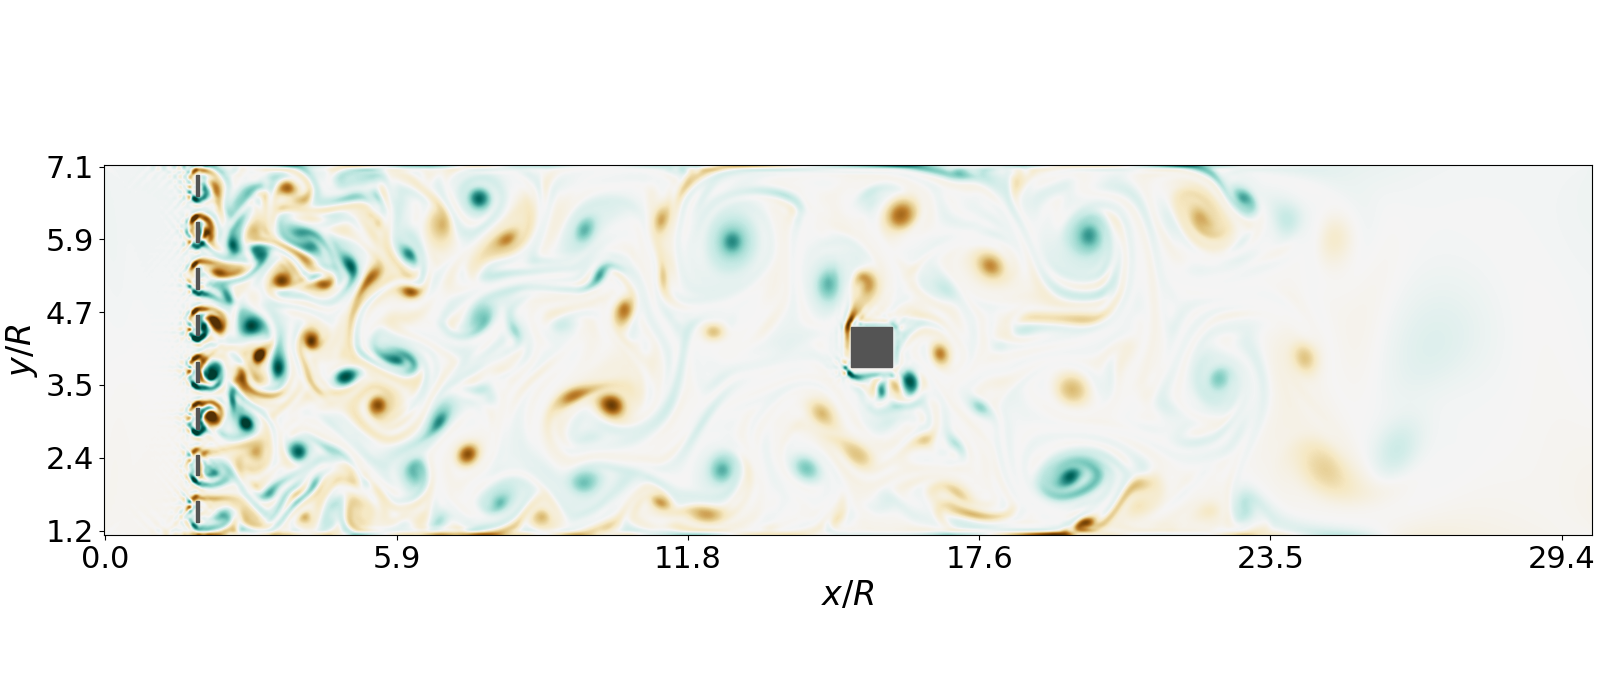
\includegraphics[width=\linewidth]{illustr_ecoulement/illustr_ecoulement}
	\caption{Our case study is a grid-generated turbulent flow impinging onto a fixed squared obstacle (of size $R$) located at the centre of a channel in two dimensions. The flow is artificially damped near the end of the channel. In the developed flow, turbulent eddies have typically the size of the square, which results in strong fluctuations of mechanical efforts acting on the square. The vorticity is displayed with an arbitrary colour map from blue (negative values) to red (positive values).}
	\label{fig:illustr_ecoulement}
\end{figure}

% introduce the flow
%
The drag exerted by a grid-generated turbulent flow onto a fixed squared obstacle is considered as a representative case study (see Fig.~\ref{fig:illustr_ecoulement}).
% why this flow?
%
Although real-world applications would eventually imply three-dimensional dynamics, a simplified two-dimensional setting has been chosen here to reduce the computational cost and allow for a systematic study.
%
We believe that this system embeds the characteristic features that makes this study challenging and relevant for fluid-structure-interaction problems.
% rapid description of the flow
Turbulent eddies generated in the near-wake of the grid are carried downstream.
They interact with each other and grow in size as expected for two-dimensional turbulent dynamics.
The dimension of the grid is such that the size of the eddies that hit the square is comparable to its size, resulting in strong fluctuations of the drag acting on the square.
%
%Finally, the obstacle does not deform or move either.
%
%Through this simplified setting, our motivation is primarily to evaluate the operability of sampling techniques to capture extreme events with a significant run-time savings.
%

% lattice Boltzmann method
%
The flow dynamics is integrated by the \ac{lbm} in our numerical simulations.
While traditional methods in computational fluid dynamics rely on a discretization of the Navier-Stokes equations, the \ac{lbm} considers the fluid at a mesoscopic level.
Capturing the dynamics of collections of fluid particles moving and colliding on a lattice is here preferred to solving non-linear PDEs.
%This seems crazy, however, most details at the mesoscopic level play actually no role at the macroscopic level. Therefore, the LB algorithm may be viewed as a minimal kinetic scheme compliant to the fluid dynamics at the macroscopic level.
Further details about the \ac{lbm} are given in Appendix \ref{app:lbm} and references therein.
In our context, this numerical method has been chosen principally for its computational manageability and efficiency.


% geometry
%
The simulated flow develops in a long plane channel of dimension $513 \times 129$ mesh points. The square obstacle has size $R=16$ (in mesh unit) and is located at the centre of the channel. The spacing and bar height of the entrance grid are both equal to $R/2$ (see Fig.~\ref{fig:illustr_ecoulement}).
% boundary conditions
%
No-slip boundary conditions are enforced on top and bottom walls of the channel and on the surface of the obstacle by using an halfway bounce-back procedure~\citep{lbm_book}.
%
Upstream of the grid, a constant parabolic velocity profile and a constant mass density (equal to unity) are imposed as an inlet condition.
The centerline velocity is $0.05$ in lattice units, \textit{i.e.} normalised by $\Delta x$ and $\Delta t$ referring to the lattice resolution and the time-step respectively. The initial distributions are imposed at equilibrium (see appendix~\ref{app:lbm}).
In the bulk, the viscosity is adjusted so that grid turbulence is generated with Reynolds number $\mathrm{Re_{grid}}=1200$. The reference Mach number is equal to $0.06$ in agreement with the assumption of weak compressibility of the \ac{lbm}.
Near the end of the channel, the flow is progressively damped within a \textit{sponge layer} where the viscosity is artificially enhanced.
Finally, the outlet boundary condition relies on a second-order extrapolation of the velocity and mass density.
The extrapolated distributions are evaluated through a regularization procedure relying on a finite difference estimation of the local stress tensor, as introduced in \cite{latt2008straight}.


\subsection{The drag force}
\label{sec:drag_force}

\begin{figure}
	\centering
	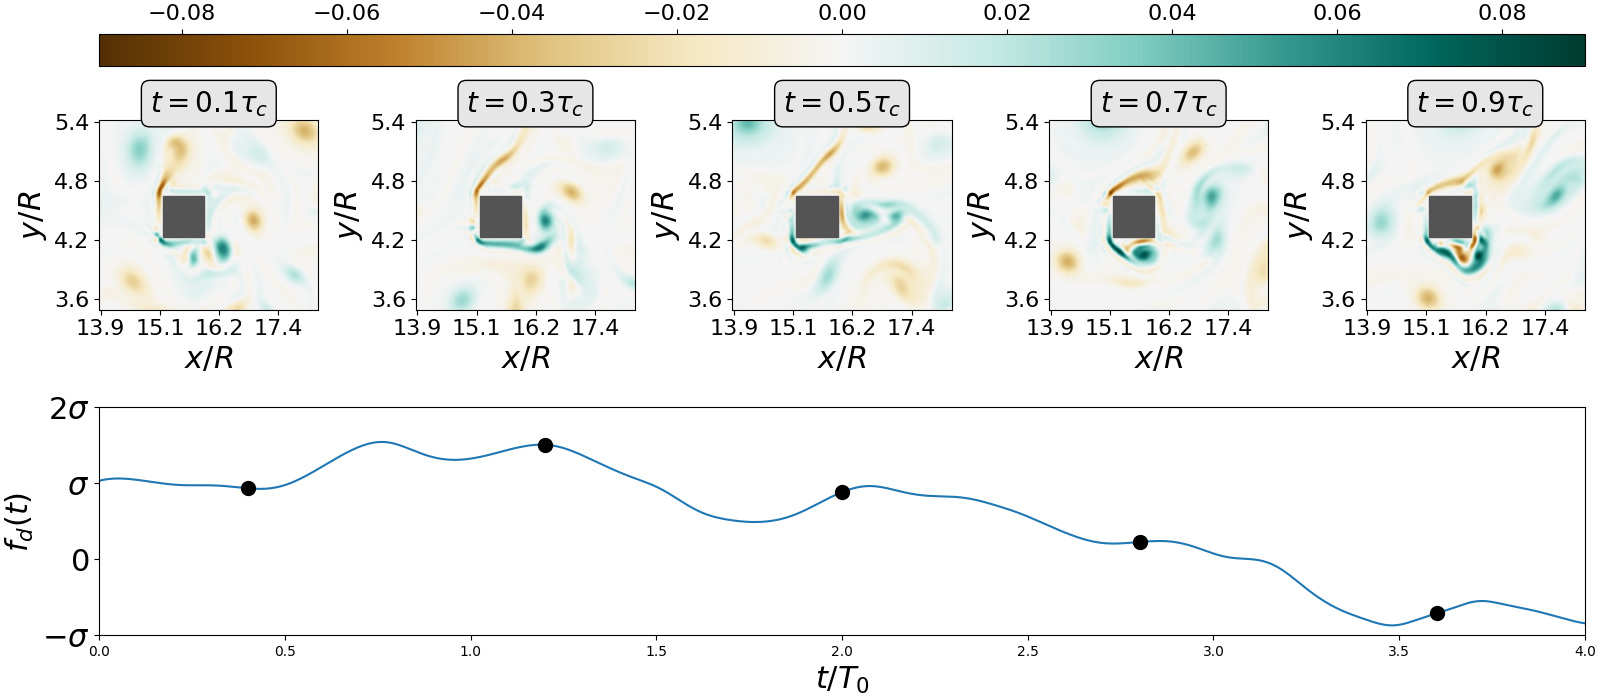
\includegraphics[width=\linewidth]{ecoulement_typique/ecoulement_typique.png}
	\caption{Snapshots of the vorticity related to typical drag fluctuations (within one standard deviation) over a time interval of length $4T_0$. The vorticity is expressed in unit of $T_0$.}
	\label{fig:typical_vorticity}
\end{figure}

%% LB parameters  %

% drag signal
%
The incoming turbulent flow exerts fluctuating mechanical efforts onto the squared obstacle.
The \textit{drag} is defined as the resulting force in the streamwise $x$-direction. Formally
\begin{equation}
\label{eq:drag_definition}
f_d(t) = \int_{\mathcal{S}} \boldsymbol{\tau}_{x \beta}(\mathbf{x},t) ~ \mathrm{d}{\mathcal{S}}_\beta(\mathbf{x}),
\end{equation}
where $\mathcal{S}$ is the surface of the obstacle and $\boldsymbol{\tau}$ denotes the stress tensor (see Appendix \ref{app:lbm})).
Here, the viscous stress makes a negligible contribution to the drag.
The latter therefore results mostly from pressure forces.
%
Since the pressure on the top and bottom sides of the square applies in the normal direction, they do not contribute to the drag.
As a consequence, the drag can eventually be expressed as the difference
\begin{equation}
\label{eq:drag_approx}
f_d(t) = p_{fb}(t) - p_{base}(t)
\end{equation}
between the pressure integrated over the upstream side of the obstacle or \textit{forebody}, $p_{fb}(t)$, and the downstream side or \textit{base} $p_{base}(t)$.
Pressure fluctuations are related to the dynamics of the vorticity field.
Regions of strong vorticity correspond to strong local pressure gradients, \emph{e.g.} as demonstrated analytically with a Rankine vortex.

% Definition of turnover time
The typical timescale (turnover time) of drag fluctuations can be estimated from dimensional analysis as
\begin{equation}
\label{eq:turnover_time}
T_0 = \frac{R}{U},
\end{equation}
where $R$ is the size of the square and $U$ is the averaged velocity in the channel.
%The viscosity is here discarded since viscous stress is negligible as compared to pressure forces.
%
% typical fluctuation of the drag
%
Fig.~\ref{fig:typical_vorticity} displays the typical evolution of the vorticity field around the obstacle over a few turnover times.
Because the vorticity generated along the forebody is swept away by the mean flow, the pressure field in the vicinity of the base is only slightly perturbed.
Vorticity is generated along the forebody and eventually carried away by the flow.
Typical fluctuations of the drag (within one standard deviation) do not result from some preferred arrangement of the vorticity around the obstacle.
\subsection{The drag as a random process
	%: Probability Density Function and correlation in time
}
\label{sec:pdfs}

\begin{figure}
	\centering
	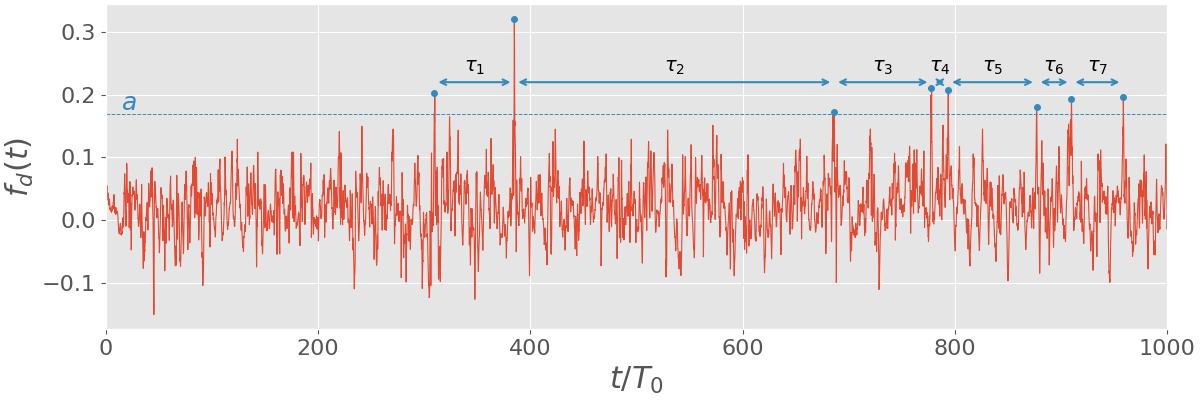
\includegraphics[width=.9\linewidth]{illustrate_return_time/illustrate_return_time}
	\caption{Temporal evolution of the drag (in lattice units) acting on the square under the action of the impinging turbulent flow. The \textit{return time} $r(a)$  is the averaged waiting time between the occurrence of peak fluctuations of amplitude larger than $a$.
          One observes that $r(a) \gg \tau_c$ (correlation time) if $a$ is sufficiently large. The selected peak fluctuations are therefore well separated.
          The time is normalised by the turnover time related the mean-flow velocity and the size of the obstacle, \emph{i.e.} $T_0=R/U$.}
	\label{fig:typical_drag_signal}
\end{figure}



% drag signal
%
% Description du signal de trainee typique
Figure~\ref{fig:typical_drag_signal} shows the time signal of the drag acting on the square, $f_d(t)$, over five hundred turnover times.
The signal appears unpredictable in details and exhibits repeated bursts of high amplitude that deviate significantly from the averaged value.
Therefore, it is natural to model the drag as a (scalar) random process.

% drag statistics
% pdf
Drag fluctuations have been sampled along a simulation of duration $T_{tot} = 4\times 10^6~T_0$.
This long simulation will be referred to as the \textit{control run} in the following.
It has been made possible by the relative simplicity of the investigated flow and the computational efficiency of the lattice Boltzmann method.
The \ac{pdf} of drag fluctuations is shown in Fig.~\ref{fig:pdf_drag_a}.
It deviates from a normal law and shows an exponential tail for large positive fluctuations, \textit{i.e.} ${\mathbb{P}}(f_d) \propto e^{-\ell f_d}$.
%
Fig.~\ref{fig:pdf_drag_a} also displays the \ac{pdf} of drag fluctuations acting on a control surface corresponding to the periphery of the obstacle but in the absence of the obstacle.
%
In that case, the \ac{pdf} is quasi-symmetric and does not display exponential tails. This shows that the asymmetry of the \ac{pdf} and the development of a positive exponential tail are closely related to the no-slip condition on the obstacle boundary.
\begin{figure}
	\centering
	\subfloat[\ac{pdf} of (zero-mean) drag fluctuations]
	{\label{fig:pdf_drag_a}
		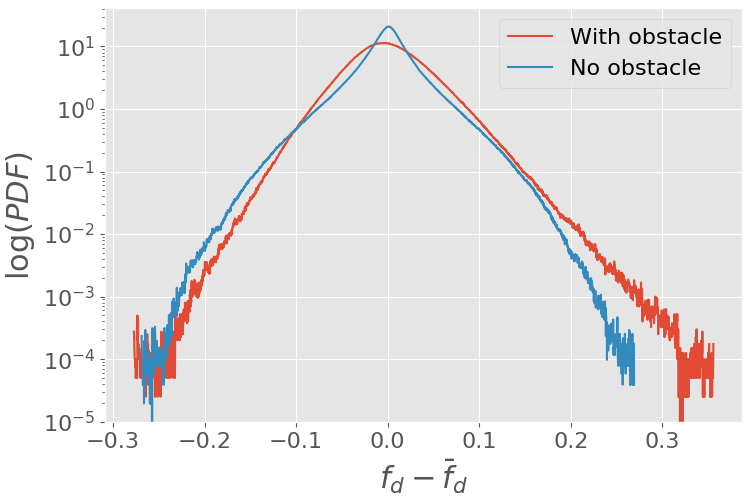
\includegraphics[width=.45\linewidth]{./PDF_drag/PDF_drag.png}}
	\subfloat[Autocorrelation of drag fluctuations]
	{\label{fig:pdf_drag_b}
		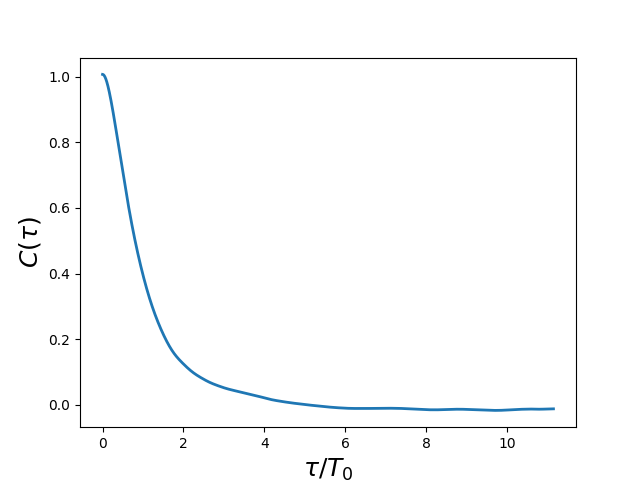
\includegraphics[width=.45\linewidth]{./autocorrelation_drag/autocorrelation_drag.png}}
	\caption{\textbf{(a)} \ac{pdf} of (zero-mean) drag fluctuations $\tilde f_d \equiv f_d - \bar{f_d}$ where $\bar{f_d}$ denotes the time-averaged value. The drag is evaluated both in the presence (red) and in the absence (blue) of the obstacle. The estimate with obstacle was computed over a timeseries spanning $4\times 10^6T_0$. The estimate without square was computed over a timeseries spanning $4\times 10^5 T_0$.
          \textbf{(b)} Autocorrelation function of the drag defined as $C(\tau) = \overline{ \tilde f_d(t+\tau)\tilde f_d(t)} ~/~ \overline{{\tilde f_d}^2}$. The correlation time $\tau_c\simeq 4 T_0$ is defined by $C(\tau_c)=0$.}
	\label{fig:pdf_drag}
\end{figure}

% drag statistics
% correlation time
Lastly, the autocorrelation function of the drag $C(\tau)$ is shown in Fig.~\ref{fig:pdf_drag_b}.
It is found that drag fluctuations are correlated over a time interval $\tau_c \simeq 4T_0$, illustrating that the drag loses its memory over a time scale corresponding to the sweeping of a few eddies past the obstacle.
%
This observation is important for the application of rare-event algorithms as it will be discussed in section~\ref{sec:rare_events_algorithms}.
%
In the following, $\tau_c$ will be referred to as the \textit{correlation time} of the drag process.
The ratio $T_0 / \tau_c$ may be viewed as a Strouhal number.
The value $St=0.25$ is consistent with common observations for flows past blunt structures at comparable Reynolds numbers \citep{rodi1998}.

%%% Local Variables:
%%% mode: latex
%%% TeX-master: "draft_p2_jfm"
%%% End:

\section{Extreme fluctuations of the drag by means of direct sampling}
\label{sec:direct_sampling}

\begin{figure}
	\centering
	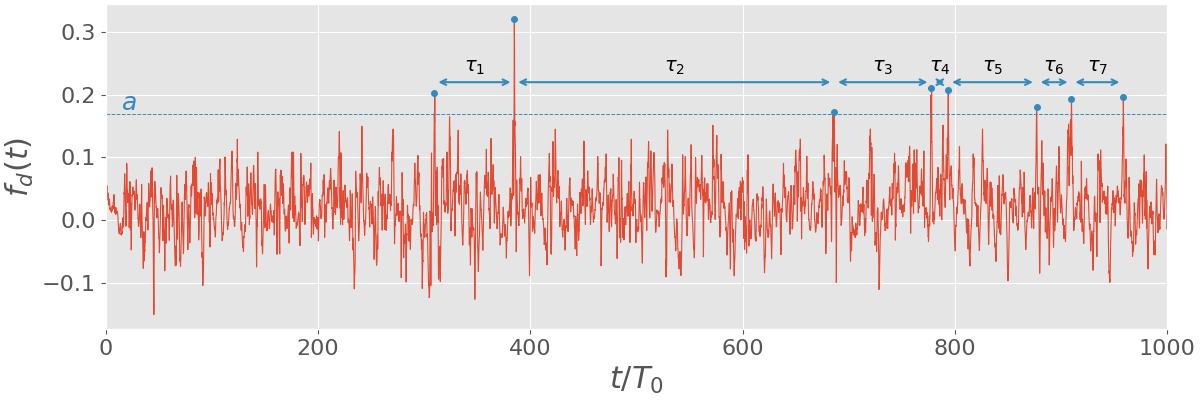
\includegraphics[width=\linewidth]{illustrate_return_time/illustrate_return_time}
	\caption{\label{fig:illustrate_return_time} {The \textit{return time} $r(a)$  is the averaged waiting time between the occurrence of peak fluctuations of amplitude larger than $a$.
            One observes that $r(a) >> \tau_c$ (correlation time) if $a$ is sufficiently large. The selected peak fluctuations are therefore well separated.}
	}
\end{figure}

\begin{figure}
	\centering
	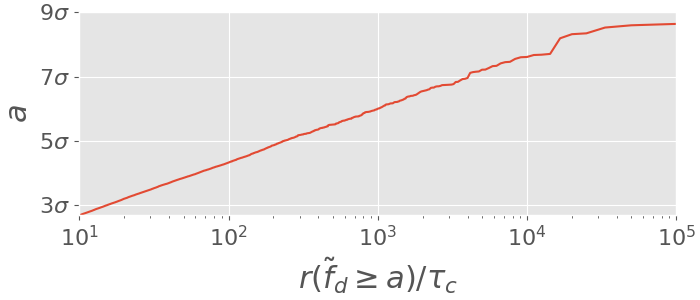
\includegraphics[width=.7\linewidth]{return_time/return_time.png}
	\caption{Amplitude of drag fluctuations as a function of the corresponding return time. $\tilde{f}_d$ denotes the drag with zero mean, \textit{i.e.} $\tilde{f}_d = f_d - \overline{f_d}$.
	}
	\label{fig:return_time_instant}
\end{figure}

% return time given from direct sampling
%
The phenomenology of extreme fluctuations of the drag is first investigated through brute-force direct sampling applied to the control run.
Direct sampling is here used as opposed to approaches involving rare-events algorithms discussed in section~\ref{sec:rare_events_algorithms}.
It will provide a trustworthy baseline for the validation of rare-events algorithms.

The waiting times $\tau$ are defined as the time between two consecutive occurrences of peak fluctuations with amplitude $f_d \geq a$, as illustrated in Fig.~\ref{fig:illustrate_return_time}.
The mixing time $\tau_m$ is the time needed for the dynamics to lose the memory of its initial condition.
As soon as the typical waiting times are much larger than the mixing time $\tau_m$, the occurrences of such events follow a Poisson process and the distribution of the waiting times is exponential, \emph{i.e.} $P(\tau)=\lambda(a)\exp(-\lambda(a)\tau)$ where $r(a)=1/\lambda(a)$ is the averaged waiting time \cite{lestang_computing_2018}; $r(a)$ is called the {\it return time} of the level $a$.
For systems without multi-stability, it is common for the mixing time $\tau_m$ to be of the order of the correlation time $\tau_c$.

How rare is a fluctuation $a$ is quantified by the return time $r(a)$.
We can define extreme drag fluctuations as \textit{rare events} in the sense that the return time is much larger than the correlation time, \emph{i.e.} $r(a) \gg \tau_c$.
%
%
If one assumes that  $r(a) = t(a)~/~\mathbb{P}(f_d\geq a)$   where the time scale $t(a)$ is of order $\tau_c$ and varies much more slowly with $a$ than ${\mathbb{P}(f_d\geq a)}$,
one might expect that
\begin{equation}
  \label{eq:return_time}
  r(a) \underset{a\to\infty}{\propto} \exp(la),
\end{equation}
where $l$ is the rate describing the positive tail of the \ac{pdf} of the drag (shown in Fig.~\ref{fig:pdf_drag}).
Fig.~\ref{fig:return_time_instant} shows the evolution of the return time $r(a)$ with the amplitude of fluctuation $a$, computed from {direct sampling} of the drag signal $f_d(t)$~\citep{lestang_computing_2018}.
Consistently, it is found that the return time $r(a)$ is well approximated by an exponential for large levels $a$. Let us also point out some deviation from the exponential law at the largest levels, which are probably the consequence of under-sampling.

% typically for $a \gtrsim 8 \sigma$ with $\sigma$ being the standard deviation.



\subsection{Extracting extreme drag fluctuations from a very long timeseries}
\label{sec:extreme_extraction}

% intro
%
We have extracted the fluctuations of the drag with a return time $r(a)$ greater than  $10^4\tau_c$ from the control time-series $\{f_d(t)\}_{0 \leq t \leq T_{tot}}$.
This set will be considered as representative of \emph{extreme events} in the upcoming study.
The choice of this particular threshold has been driven by the need to collect enough events with large amplitude and possibly identify generic features.
%
According to Fig.~\ref{fig:return_time_instant}, the related amplitude $a$ is found equal to $7.6~\sigma$ with $\sigma$ being the standard deviation of the drag process.
Precisely, 104 independent fluctuations with $f_d(t) \geq 7.6\sigma$ have been identified. Each fluctuation is characterized by its maximal value, $f_d^{\star}$, and the time, $t^{\star}$, at which this maximum is reached.
%
In the following, the phenomenology of extreme drag fluctuations will be examined on the basis of this set of events.

\subsection{Extreme fluctuations of the instantaneous drag}
\label{sec:instantaneous_drag}

\subsubsection{Contribution of forebody and base pressure fluctuations to the overall drag fluctuation}
\label{sec:forebody_and_base_contribution}

\begin{figure}
	\centering
	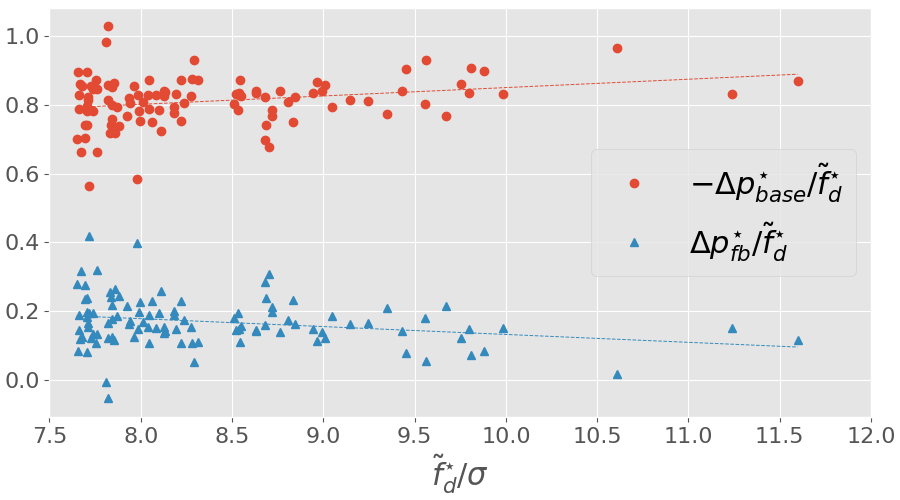
\includegraphics[width=.8\linewidth]{pressure_ratio/pressure_ratio.png}
	\caption{\label{fig:pressure_ratio} Relative contributions of the forebody and base pressure variations to extreme amplitudes of the drag. An extreme event corresponds to an amplitude $\tilde f^{\star}_d$ and a unique pair  ($\tilde{p}^{\star}_{base}$,~$\tilde{p}^{\star}_{fb}$).}
\end{figure}

% teasing
%
In section~\ref{sec:test_flow}, it was pointed out that drag fluctuations within one standard deviation were not associated with any particular arrangement of the vorticity around the obstacle.
In the following we show that the situation os different in the case of extreme drag fluctuations.

% relative contribution of forebody and base pressure
%
Let $(t^{\star}, f_d^{\star})$ refer to an extreme-drag event.
The (zero-mean) fluctuation $\tilde{f}_d^{\star} = f_d^{\star} - \overline{f_d}$ can be  decomposed into
\begin{equation}
\tilde{f}_d^{\star} = \Delta p_{fb}^{\star} - \Delta p_{base}^{\star}
\end{equation}
where $\Delta p_{fb}^{\star}$ and $\Delta p_{base}^{\star}$ denote the variations of the forebody and base pressure, respectively.
%
Fig.~\ref{fig:pressure_ratio} displays the relative contributions
$\Delta p_{fb}^{\star}/\tilde{f}_d^{\star}$ and $-\Delta p_{base}^{\star}/\tilde{f}_d^{\star}$ to the drag fluctuation $\tilde f_d^{\star}$.
It is found that very large fluctuations of the drag result mainly ($\sim 80\%$) from the drop of the base pressure, whereas the variation of forebody pressure contributes much less to $\tilde{f}_d^{\star}$.
On the contrary, moderate fluctuations arise from combined variations of the forebody and base pressures without any particular predominance, which is in agreement with the previous observations (see Fig.\ref{fig:typical_vorticity}).

\subsubsection{Fluid dynamics related to extreme drag fluctuations}
\label{sec:dynamical_aspects}

\begin{figure}
	\centering
	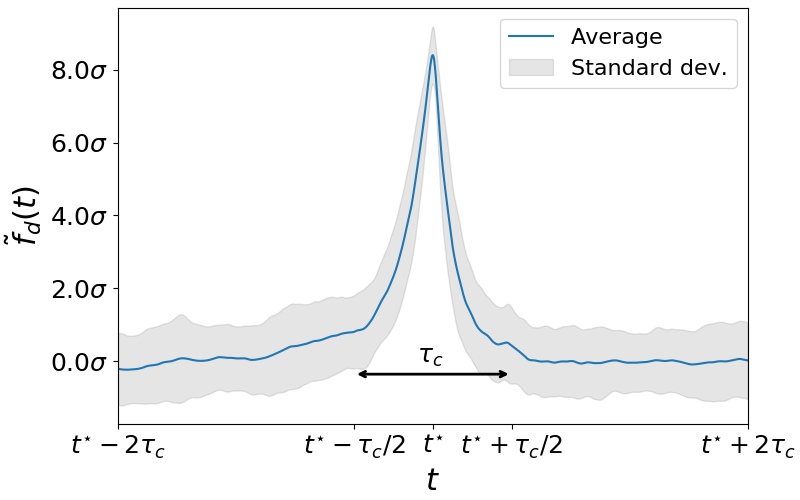
\includegraphics[width=.7\linewidth]{timeseries_extremes/timeseries_extremes.png}
	\caption{\label{fig:timeseries_extremes} Ensemble average of drag signals centred around extreme fluctuations occurring  at $t=t^{\star}$. The blue line shows the mean profile whereas the shaded area indicates variations (around the mean profile) within one standard deviation. Extreme-drag events exhibit a typical lifetime of one correlation time $\tau_c$. The profile is slightly skewed indicating that the step up is slower than the return to typical values.}
\end{figure}

% mean profile around burst
%
The focus is now on the flow scenarii that yield extreme values of the drag.
Fig.~\ref{fig:timeseries_extremes} displays the mean profile (in time) of the drag signal around extreme events. A peaked profile is observed with a width roughly corresponding to one correlation time $\tau_c$. This shows that the duration of extreme events corresponds typically to the sweeping time of the flow past the obstacle.
%Starting from typical values, extreme drags are typically reached in less than a correlation time.
Interestingly, the profile is also slightly skewed indicating that the step up of the drag is slower than the return to typical values past the peak value.
%This is reminiscent of time-irreversibility in turbulent dynamics.
This asymmetry (under time reversal) is closely linked to the symmetry breaking in what happens before and after the obstacle.
To better understand the flow scenarii leading to these events, the vorticity fields around the obstacle are now examined.

\begin{figure}
  \centering
  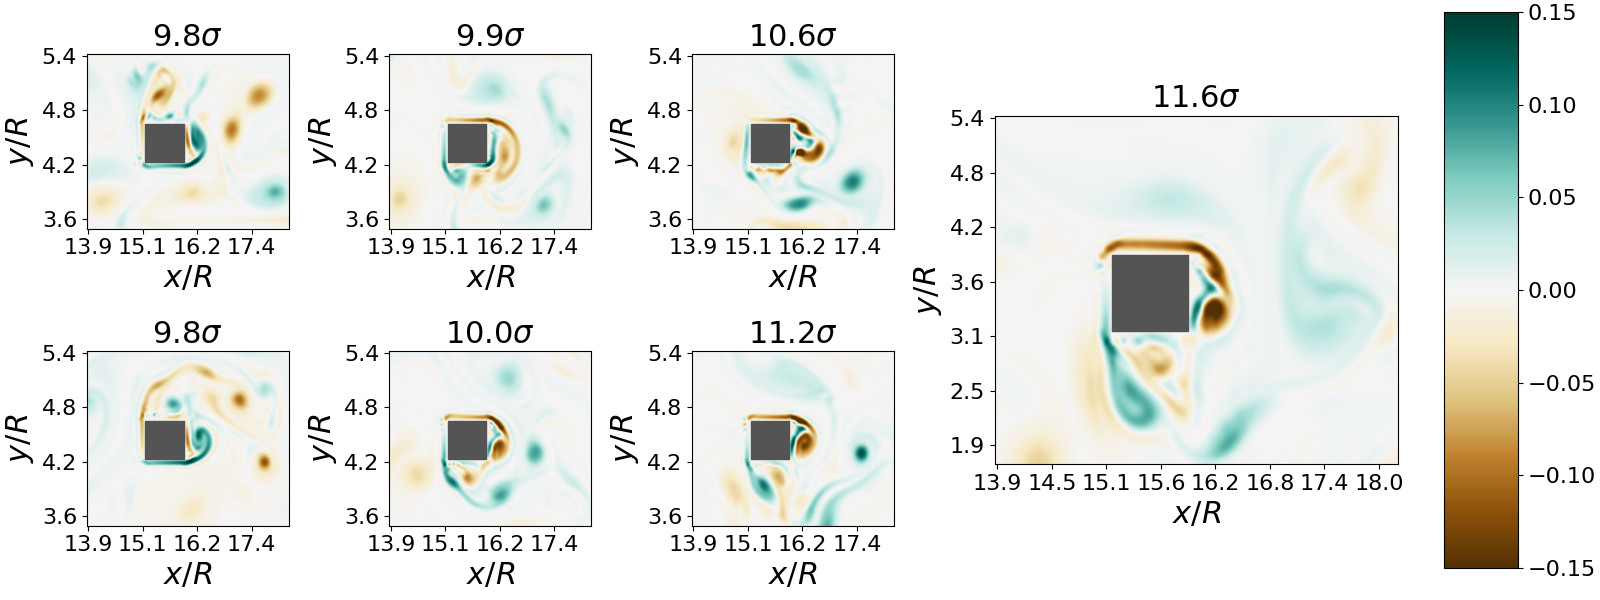
\includegraphics[width=\linewidth]{illustr_extrms_vorticity/illustr_extrms_vorticity.png}
  \caption{\label{fig:top_4_events_vorticity} Vorticity field (in lattice units) around the obstacle at $t=t^{\star}$ for the highest drag amplitudes recorded in the control run.
  }
\end{figure}

\begin{figure}
  \centering
  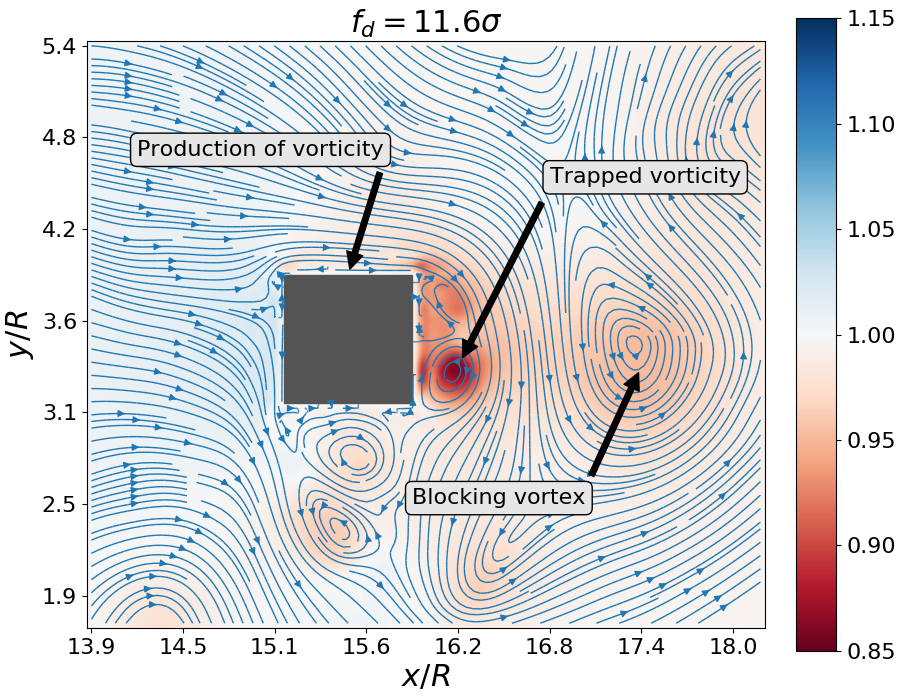
\includegraphics[width=.5\linewidth]{illustr_density_streamlines/illustr_density_streamlines.png}
  \caption{\label{fig:density+streamlines} Pressure field (in lattice units) and velocity streamlines at $t=t^{\star}$. In the near wake of the square, a (blocking) vortex blocks an intense vortex against the base of the obstacle.}
\end{figure}

\begin{figure}
  \centering
  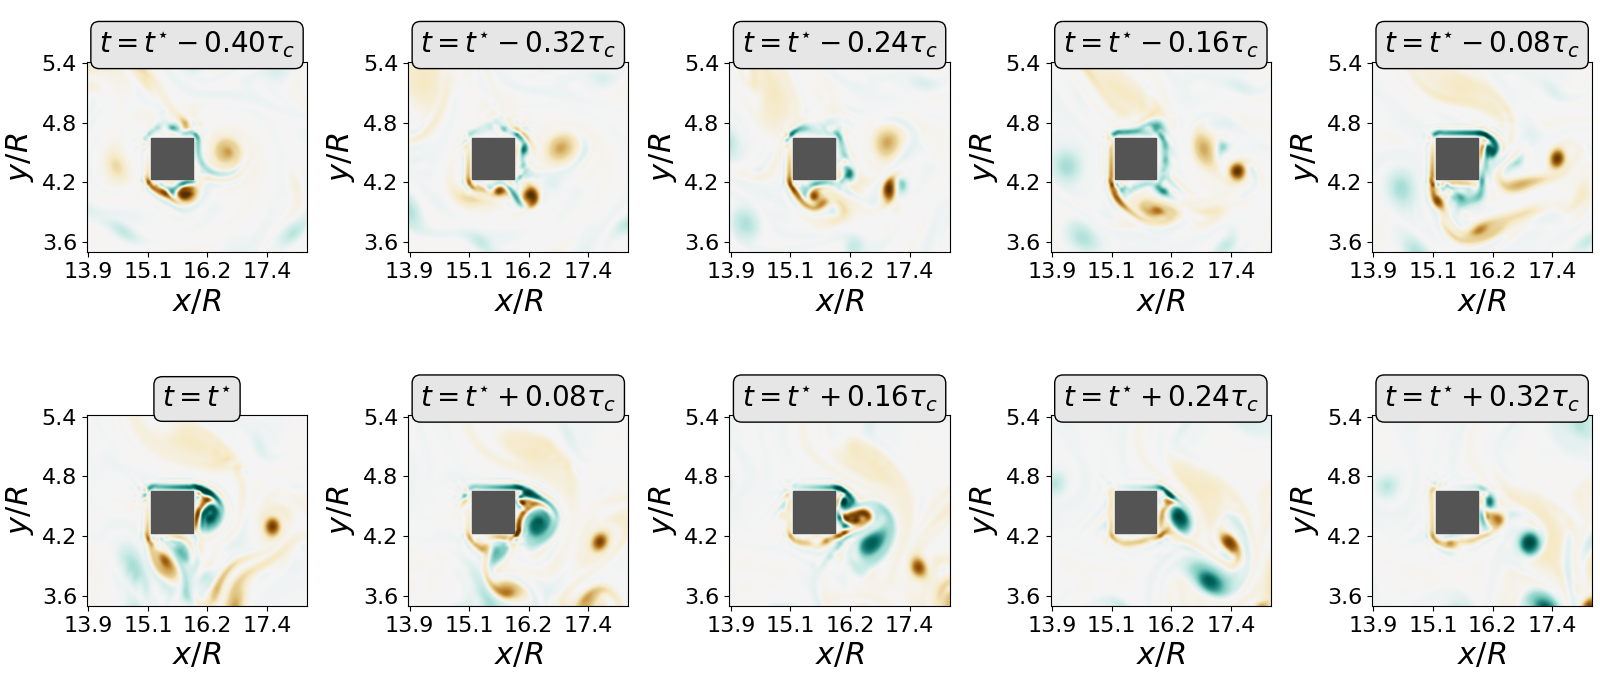
\includegraphics[width=.8\linewidth]{dynamics_extremes/dynamics_extremes.png}
  \caption{\label{fig:vorticity_dynamics} Snapshots of the vorticity field (in lattice units)  around $t=t^{\star}$.}
\end{figure}
% flow scenario
%
Fig.~\ref{fig:top_4_events_vorticity} displays the vorticity field (in lattice units) around the obstacle for the highest amplitudes of the drag during the control run.
%
In each case, an intense vortical structure is visible near the base of the obstacle.
The vorticity level of this structure is typically twice the amplitude of typical vorticity fluctuations observed in Fig.~\ref{fig:typical_vorticity}.
%+
The formation of this vortex originates from an intense negative (or positive) vorticity layer at the top (or bottom) boundary of the obstacle.
%
This high vorticity is responsible for a significant pressure drop at the base of the obstacle and therefore a strong drag.
In contrast, nothing special happens near the forebody of the obstacle during extreme-drag events.

The high pressure drop near the base of the obstacle appears to be closely related to the presence of a strong vortex blocked against the base.
As illustrated in Fig.~\ref{fig:density+streamlines}, this blockage is enforced by the presence of opposite vorticity in the near wake, which holds the vortex against the base of the obstacle and prevents it from being swept away for a while.
%
This scenario is better evidenced by Fig.~\ref{fig:vorticity_dynamics}, where the time history of the vorticity field around $t=t^\star$ for the same event is shown.
%
Before the occurrence of the extreme event, positive vorticity originating from the bottom boundary layer develops in the near wake of the square. This positive vorticity  prevents the shedding of negative vorticity and enforces the development of a intense vortex against the base of the square.
As the blocking vortex is in turn advected downstream, the vortex against the base is released.
%
Consistently, one can argue that the typical duration of this scenario is related to the sweeping time of the flow past the obstacle, and is therefore of the order of $\tau_c$.
This is in full agreement with the typical duration obtained from statistical consideration on the mean profile of large-drag fluctuations in Fig.~\ref{fig:timeseries_extremes}.
This scenario is generic and has been observed for most extreme events sampled in the control run.

%We found that $80\%$ of the extreme events sampled from the control timeseries can be related to very similar dynamics.

\begin{figure}
  \centering
  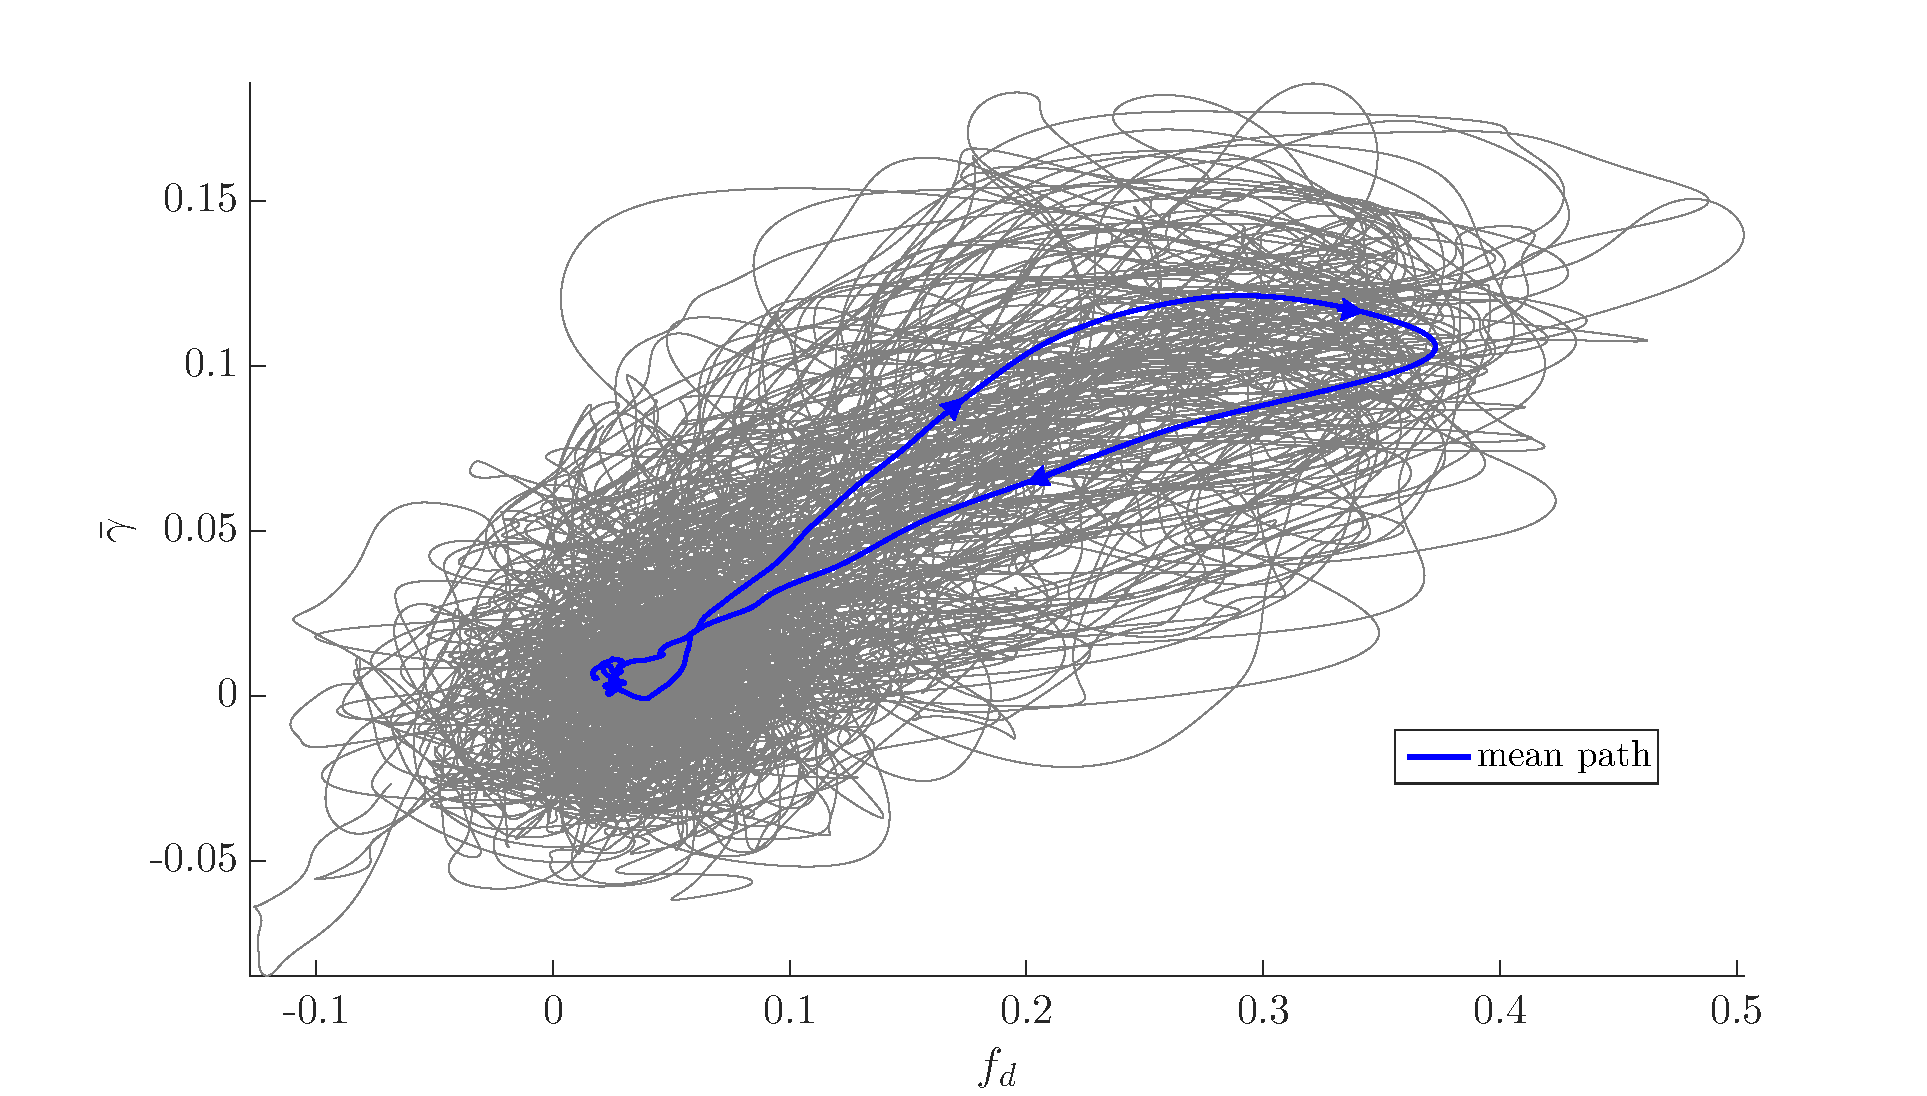
\includegraphics[width=.7\linewidth]{shear_asof_drag/shear_asof_drag}
  \caption{\label{fig:shear_asof_drag} Evolution of the (integrated) shear along the top or bottom sides of the obstacle as a function of the drag for $t^{\star}-2\tau_c \leq t \leq t^{\star}-2\tau_c$. Each trajectory corresponds to a single event. The blue line is the mean path averaged over the set of extreme events sampled in the control run.}
\end{figure}

Since the occurrence of large drag amplitudes arises from the production of vorticity along the top or bottom side of the square, it is proposed to characterize the dynamics of extreme events by their trajectory in the parameter space $(f_d(t), \bar{\gamma}(t))$ where $\bar{\gamma}(t)$ is the averaged shear along the top or bottom boundary of the square:
\begin{equation}
\label{eq:avg_shear_def}
\overline{\gamma} = \frac{1}{R} \int_{\mathcal{S}_\parallel} \frac{\partial u(\mathbf{x})}{\partial y}\mathrm{d}\mathbf{x},
\end{equation}
where $R$ denotes the size of the square, $u$ is the streamwise component of the velocity field and $\mathcal{S}_\parallel$ is the surface of either the top or the bottom boundary.
%
Fig.~\ref{fig:shear_asof_drag} shows $\overline{\gamma}(t)$ as a function of the instantaneous drag $f_d$(t) for $t^{\star}-2\tau_c \leq t \leq  t^{\star}+2\tau_c$ for the 104 sampled extreme events.
Before and after the extremal fluctuation, \textit{i.e.} for $t^{\star}-2\tau_c \leq t \leq t^{\star}-\tau_c$ and $t^{\star}+\tau_c \leq t \leq t^{\star}+2\tau_c$, paths wander in a region related to typical values of both $\overline{\gamma}$ and $f_d$.
On the contrary, the drag abruptly varies for $t^{\star}-\tau_c \leq t \leq t^{\star}+\tau_c$ near the extremal amplitude.
%Paths in the $(f_d, \bar{\gamma})$ space display excursions to atypical values for both $\bar{\gamma}$ and $f_d$.
These excursions always go clockwise, that is, $\overline{\gamma}$ attains its maximum value before $f_d$ does.
This is consistent with an increase of $\overline{\gamma}$ acting as a precursor for extreme drag fluctuations.
In this representation, we also observe that the path related to the increase of the drag is longer than the path related to the return to typical values.

\subsection{Extreme fluctuations of the time-averaged drag }
\label{sec:time_avg}

\begin{figure}
	\centering
	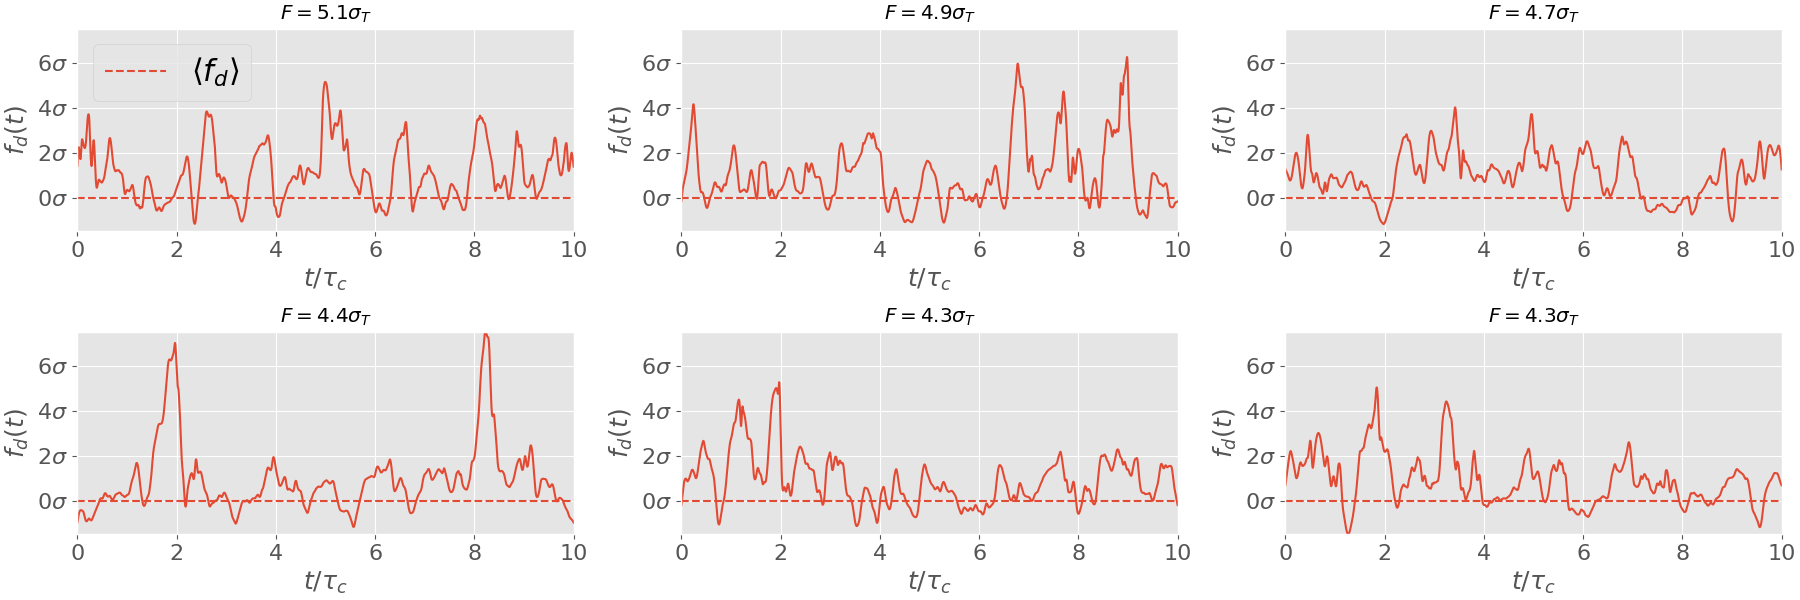
\includegraphics[width=\linewidth]{timeseries_extrms_AVG/timeseries_extrms_AVG}
	\caption{Instantaneous drag signals $f_d(t)$ corresponding to the highest fluctuations of the averaged  drag $F_T$ with a time window $T = 10 \tau_c$;  $\sigma$ and $\sigma_T$ denote the standard deviations of the instantaneous and averaged drag, respectively.}
	\label{fig:extreme_avg}
\end{figure}


% motivation
%
%In section~\ref{sec:instantaneous_drag}, we discussed the phenomenology of rare events corresponding to extremely high values of the drag acting on the square obstacle mounted in the flow described in section~\ref{sec:test_flow}. In particular, it was pointed out that such extreme drag fluctuations have a lifetime of, roughly, one correlation time $\tau_c$.

%We discussed previously the phenomenology of extreme fluctuations of the \emph{instantaneous} drag and pointed out that the time scale associated with the development of such event is of the order of the sweeping time of the flow past the obstacle $\tau_c$.
We discussed previously the phenomenology of extreme fluctuations of the \emph{instantaneous} drag, and identified the sweeping time of the flow past the obstacle as the characteristic lifetime of these events.
%
In applications, this duration may be much smaller than the response time of the material structure subject to these fluctuations, justifying a practical interest in the averaged (in time) drag force.
% Consider for instance the interaction of a deformable structure with a turbulent flow: the typical response time may be much larger than the lifetime of drag fluctuations.
%
% definition
%
Therefore, a relevant observable is the \textit{time-averaged} drag defined as
\begin{equation}
\label{eq:def_time_averaged_drag}
F_T(t) = \frac{1}{T}\int_t^{t+T} f_d(t) \mathrm{d}t,
\end{equation}
where $f_d(t)$ denotes the instantaneous drag and $T$ is the investigated timescale (response time).
In the following, we shall consider $T=10\tau_c$, where $\tau_c$ is the correlation of the instantaneous drag.
In that case, the PDF of $F_T$ is found nearly Gaussian as a consequence of the Central Limit theorem (see Fig.~\ref{fig:IS_GKTL}).

%
During a time interval $[t;t+T]$, a fluctuation of $F_T(t)$ may be roughly viewed as the overall contribution of  $T / \tau_c$ independent fluctuations of the {instantaneous} drag $f_d$.
% phenomenology
%
% What is the phenomenology leading to extreme values of $F_T(t)$ ?
It is thus legitimate to ask whether a large value of the averaged drag results from a single outstanding fluctuation of the instantaneous drag (case (1)),  or from  an unusual succession of moderate positive fluctuations (case (2)).
%
In the same way as in section \ref{sec:extreme_extraction}, one can identify extreme fluctuations of $F_T$ exceeding some fixed threshold $a$, and sample a set of extreme events.
By taking $a=5.2\sigma_T$ with $\sigma_T$ being the standard deviation of $F_T$, $84$ independent extreme events have been selected.
Again, this choice results from a compromise between the need to consider large deviations from the mean value and the requirement to sample a sufficient number of events for meaningful statistics. As a rule of thumb, the threshold has been set so that around one hundred events are selected.


% neither case (1) nor case (2)
%
Fig.~\ref{fig:extreme_avg} displays the time-series $\{f_d(t)\}_{t^{\star} \leq t \leq t^{\star}+T}$ for several extreme fluctuations of $F_T$ occurring at $t=t^\star$.
Qualitatively, it is found that extreme fluctuations of the time-averaged drag can neither be reduced to case (1) nor case (2).
Indeed, both cases are %equally
featured in Fig.~\ref{fig:extreme_avg};
very large value of the averaged-drag appear to result from either a very large fluctuation, or a significant succession of moderate (positive) fluctuations of the instantaneous drag.

%%% Local Variables:
%%% mode: latex
%%% TeX-master: "draft_p2_jfm"
%%% End:

\section{Rare-events algorithms}
\label{sec:rare_events_algorithms}

According to Eq.~\eqref{eq:return_time}, the return time of fluctuations $f_d \geq a$ scales like
$r(a)\propto e^{l a}$, meaning that the computational cost required to sample events of amplitude $f_d \geq a$ through brute-force sampling diverges exponentially.
The direct sampling approach used in the previous sections to sample extremes of the drag is therefore not scalable and it would be difficult, if even feasible, to study rarer events or more complex flows.

In this section, we investigate the use of rare-events algorithms in order to sample extreme events for a
computational cost much lower than their return time.
Should this approach be successful, it would pave the way to the simulation of extreme events for flows of
greater complexity than the two-dimensional flow discussed in the previous sections.

We focus on two algorithms, representatives of two popular approaches in rare event simulation.
The first one is the \acl{ams} algorithm \citep{cerou_adaptive_2007} and builds on previous ideas about splitting approaches \citep{KahnHarris1951,glasserman_multilevel_1999}.
In recent years, it has allowed for the computation of rare events in problems involving a large number of degrees of freedom, such as molecular dynamics simulations \citep{aristoff_adaptive_2015,teo_adaptive_2016} or stochastic partial differential equations for the computation of rare trajectories in the Allen-Cahn equations \citep{rolland_computing_2016}. More recently, it has been applied to rare events in stochastic models of wall-turbulence \citep{rolland_extremely_2018} and atmospheric dynamics \citep{bouchet2019rare}.
The second algorithm we consider in this section is the cloning algorithm \citep{giardina_direct_2006}, also known as population dynamics or interacting particles system algorithm.
This approach is very similar to the Diffusion Monte Carlo method used in computational chemistry, and has been introduced and refined in many variants.
Among them the cloning algorithm introduced by Giardina and Peliti \citep{giardina_direct_2006} was successfully applied to chaotic dynamical systems \citep{giardina_simulating_2011,Laffargue_2013}.
More recently it allowed the numerical simulation of extreme heat waves in a simplified model of the atmosphere \citep{ragone_computation_2018}.
This use represents a significant leap in the applicability of rare-event sampling algorithms to complex dynamical systems.
Along the same line, rare-event sampling algorithms are here applied outside of traditional applications by considering fluid-structure interaction in a turbulent flow.

The \ac{ams} is based on the simulation of an ensemble of $N$ independent trajectories $\{\mathbf{x}_n(t)\}_{0\leq t \leq T_a}$ with $n=1 \cdots N$.
Each $\{\mathbf{x}_n(t)\}_{0\leq t \leq T_a}$ refers to a trajectory of duration $T_a$ in the phase space of the
system.
Following the initial simulation of this ensemble, trajectories are iteratively resampled in order to maximise the maximum value of a score function $\xi(\mathbf{x})$ along the trajectories.
The difficulty in applying the \ac{ams} lies in the choice of the score function, which can drastically
influence the effectiveness of the resampling in leading to extreme events \citep{rolland_statistical_2015}.
Mathematical analysis of the \ac{ams} provide proof of existence of an optimal score function, kown as the
committor function. However, with the exception of rare analytical cases, this function is unknown.
See appendix~\ref{app:AMS_on_OU} for a description of the \ac{ams} and its basic mathematical properties.

Similarly to the \ac{ams}, the cloning algorithm simulates an ensemble of trajectories of the system.
However, resampling steps are performed along the simulation of the ensemble.
Trajectories are first evolved independently from $t = 0$ to $t=\tau < T_a$ and then duplicated or pruned
according to the average of an observable $O(\mathbf{x})$ over the interval $[0;\tau]$.
This procedure is then repeated $n-1$ times over the intervals $[\tau, 2\tau], [2\tau, 3\tau]... [(n-1)\tau, n\tau = T_a]$.
Ultimately, the sampled trajectories are distributed according to a probability distribution that is tilted towards large values of the average observable:
\begin{align}
\mathbb{P}_{k}\left(\left\{ \mathbf{X}(t)\right\} _{0\leq t\leq T_{a}}=\left\{ \mathbf{x}(t)\right\} _{0\leq t\leq T_{a}}\right) &\underset{N\rightarrow\infty}{\sim} \frac{e^{k\int_{0}^{T_{a}}O(\mathbf{x}(t))dt}}{Z(k,T_a)}\mathbb{\mathbb{P}}_{0}\left(\left\{ \mathbf{X}(t)\right\} _{0\leq t\leq T_{a}}=\left\{ \mathbf{x}(t)\right\} _{0\leq t\leq T_{a}}\right),
\label{eq:Biased_Path_Approximation_main}
\end{align}
where
$\mathbb{P}_{0}\left(\left\{ \mathbf{X}(t)\right\} _{0\leq t\leq T_{a}} = \left\{ \mathbf{x}(t)\right\} _{0\leq t\leq T_{a}}\right)$ refers formally to the probability of observing the trajectory
$\left\{ \mathbf{x}(t)\right\} _{0\leq t\leq T_{a}}$ according to the unbiased statistics of the model.
See appendix~\ref{app:gktl} for a more detailed description of the cloning algorithm.

Both algorithms are similar in the way that they evolve an ensemble of trajectories, introducing selection
rules to bias the sampling towards extreme events.
In both cases, the output of the algorithm is an ensemble of $N$ trajectories that over-samples the extreme
events of interest.
Note that these trajectories are not statistically independent, however rigorous mathematical results link the statistics sampled by the algorithms to the unbiased statistics of the system, \textit{i.e.} the statistics sampled by a direct sampling approach \citep{DelMoral2013, brehier:hal-01142704}.

Most previous applications of the \ac{ams} and cloning algorithm target stochastic dynamics.
We stress that this is not the case in this work, as the target flow model is fully deterministic.
Because in both algorithms the initial condition of resampled trajectories is taken as the flow state of another, it is therefore required to add a random perturbation to the initial conditions of resampled trajectories, so that they separate from the trajectory they are resampled from.
The amplitude of this perturbation is chosen very low, and it was tested that it does not impact the statistics of the sampled trajectories.
The separation of trajectories under this slight perturbation is guaranteed by the chaoticty of the flow.
For further details about the addition of this perturbation, see appendix~\ref{app:perturb_branching_time}.

\subsection{The \acl{ams} algorithm}
\label{sec:ams}
We applied the \ac{ams} algorithm, described in appendix\ref{app:ams}, to the sampling of extreme fluctuations of the drag applied on the square obstacle immersed in the flow described in section~\ref{sec:test_flow}.
We chose to set the score function as the drag itself, that is $\xi(\mathbf{x}) = f_d(\mathbf{x})$.
Let us stress that we do not expect this choice to be close to the optimal "committor" function.
Because of the complexity of the dynamics, approaching the optimal score function requires intricate insight
into the physics that lead to the extreme events of interest.
Considering further application of the \ac{ams} to complex, three-dimensional flows, such knowledge is out of reach.
It is therefore important to assess the relevance of the application of the algorithm based on a naive choice for the
score function, a choice that is often the only available one.

In addition to the score function, the parameters of the \ac{ams} are the number of trajectories $N$ and the duration of trajectories $T_a$.
As detailed in appendix~\ref{app:ams}, the size of the ensemble $N$ governs the statistical error affecting the estimators based on the sampled set of trajectories.
Furthermore, the number of resamplings required to reach a final ensemble of trajectories of probability of the order of $10^{-\beta}$ can be shown to scale like $\beta N$ \citep{lestang_computing_2018}.
In this work, the choice of $N$ was governed by the available computational resources.
We performed two experiments with $N = 32$ and $N = 256$, having in mind that higher numbers are unlikely to be accessible in the case of more complex or three-dimensional flows.
The duration of the trajectories was set to $T_a$ = $5\tau_c$, a value that is larger than the timescale of extreme drag fluctuations whilst maintaining an affordable computational cost.
As pointed out in appendix~\ref{app:ams}, setting $T_a \gg \tau_c$ does not lead to a better sampling.

\begin{figure}
  \centering
  \subfloat[\label{fig:AMS_drag_trajectories_a} Final ensemble of trajectories sampled by the \ac{ams}]{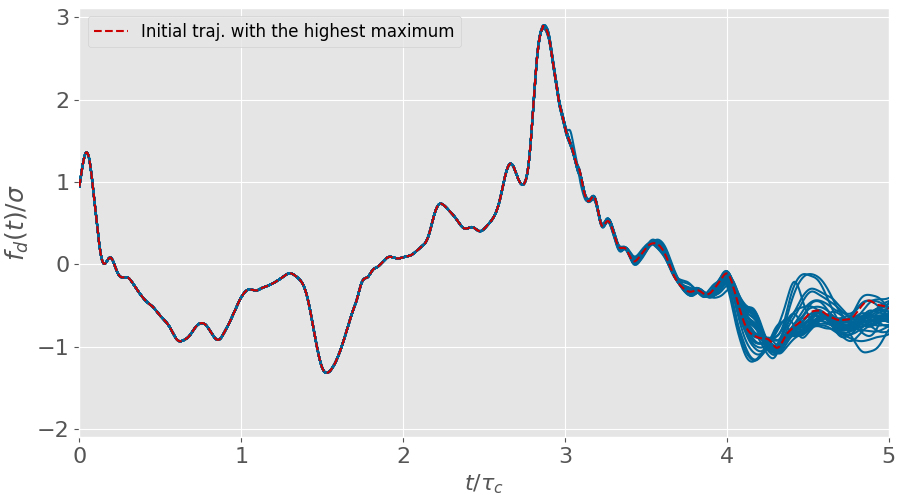
\includegraphics[width=.4\linewidth]{AMS_drag_trajectories/AMS_drag_trajectories.png}}
  \subfloat[Drag maximum for resampled trajectories]{\label{fig:AMS_drag_trajectories_b}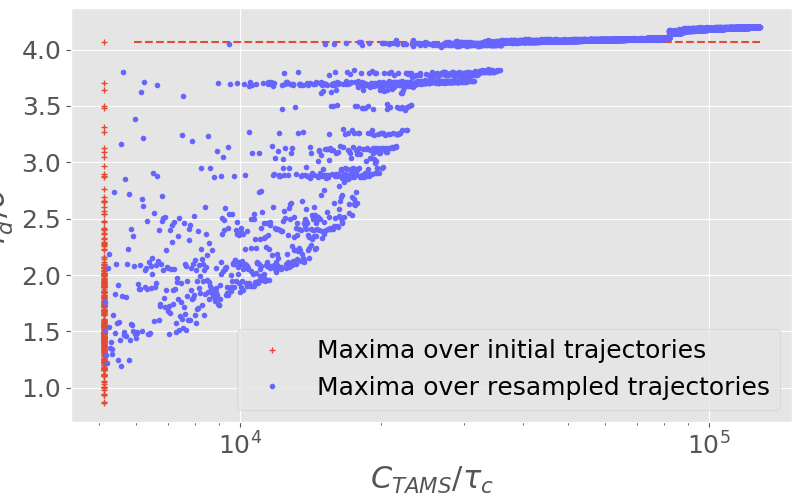
\includegraphics[width=.4\linewidth]{AMS_drag_resampling/AMS_drag_resampling.png}}
  \caption{(a) Ensemble of $N = 32$ trajectories after $181$ \ac{ams} resamplings.
    (b) Maximum of the instantaneous drag throughout the resampled trajectories as a function of the corresponding computational cost $C_{AMS}$, \textit{i.e.} as a function of the resamplings. The maximum over resampled trajectories overlap until saturating at the level of the largest maximum in the initial ensemble.
  }
\end{figure}

Figure~\ref{fig:AMS_drag_trajectories_a} illustrates that the splitting introduced by the \ac{ams} does not enhance the sampling of extremes but rather has catastrophic consequences on the sampling of trajectories.
Indeed, trajectories in the final ensemble overlap over most of their duration and are replicates of the trajectory presenting the largest maximum in the initial ensemble.
This result is confirmed by increasing the number of initial trajectories from $N=32$ to $N=256$, as shown
in figure~\ref{fig:AMS_drag_trajectories_b}.
Recalling section~\ref{sec:instantaneous_drag}, extreme drag fluctuations have a lifetime of $\tau_c$, the timescale over which a vortex is blocked near the base of the obstacle.
After $\tau_c$, the vortex is freed and swept downstream, and further large drag fluctuations can only result from the interaction of the obstacle with the incoming flow, beyond the correlation time of the drag fluctuations.
Moreover, it takes a certain time $\tau_L$ (known as the Lyapunov timescale) before a trajectory resampled by the \ac{ams} separates from its parent under the effect of the initial perturbation.
In our situation, this ``memory effect'' originates from the fact that the score function is of dimension much smaller (here 1) than the dimension of the phase space (very large for this fluid dynamics problem).
%
We observe in Fig.~\ref{fig:AMS_drag_trajectories_a} that this separation timescale is larger than the duration of extreme drag fluctuations $\tau_c$, leading to an overlap of trajectories.

We stress that this phenomenology is independent of the choice of $N$ and $T_a$.
Increasing the size of the initial ensemble can only increase the amplitude of the the global maximum attained initially, but does not solve the issue of overlapping trajectories.
Increasing $T_a$ allows further time for resampled trajectories to develop rare fluctuations, however after a duration $\Delta T \geq \tau_L > \tau_c$, and therefore decorrelated from the resampling.

Our results indicate that the \ac{ams} does not work with this simple choice of score function.
Better results may be obtained by using a different score function, but at this stage we do not know how to build such a score function for this specific problem.

\subsection{The \ac{gktl} algorithm}
\label{sec:gktl}
We applied the cloning algorithm described, in appendix\ref{app:gktl}, to the two-dimensional flow described in section~\ref{sec:test_flow}.
Unlike the case of the \ac{ams} in section~\ref{sec:ams}, the algorithm is here used to sampled trajectories that exhibit extremes values of
the \emph{average} drag.

The cloning algorithm depends on three parameters: the cloning strength $k$, the number of trajectories $N$ and the resampling period $\tau$.
The cloning strength is the multiplicative factor appearing the the bias term of equation~\eqref{eq:Biased_Path_Approximation_main}.
The higher $k$, the larger the typical average drag for the trajectories in the ensemble sampled by the algorithm.
There is however no general relation between this typical value and the value of $k$, and this value must be set empirically.
Similarly to the \ac{ams}, $N$ governs the error affecting estimates of probabilities and estimators based on the biased ensemble.
In the cloning algorithm, the population of trajectories is periodically resampled as the trajectories are simulated from $t=0$ to
$t=T_a$.
The cloning period determines how often this resampling step is performed.
For deterministic dynamics, a common rule of thumb is to chose $\tau \approx \tau_c$ \citep{giardina_direct_2006}.
For further details about the cloning algorithm, see appendix~\ref{app:gktl}.

In practice, we started by fixing the computational cost associated with a single run of the cloning algorithm, \textit{i.e.} by fixing $N \times T_a$.
Consistently with section~\ref{sec:time_avg}, we aim at sampling trajectories with a duration $T = 10\tau_c$.
Consequently, we fixed $T_a = 15\tau_c$ to allow for an initial transient regime of the cloning algorithm.
Then, we chose $N = 1024$ to obtain a computational cost of order $\mathcal{O}(10^4 \tau_c)$, \textit{i.e.} roughly one hundredth of the computational cost associated with the direct numerical simulation used for direct sampling in section~\ref{sec:direct_sampling}.
Finally, we set $\tau = \tau_c / 2$.

\begin{figure}
  \centering
  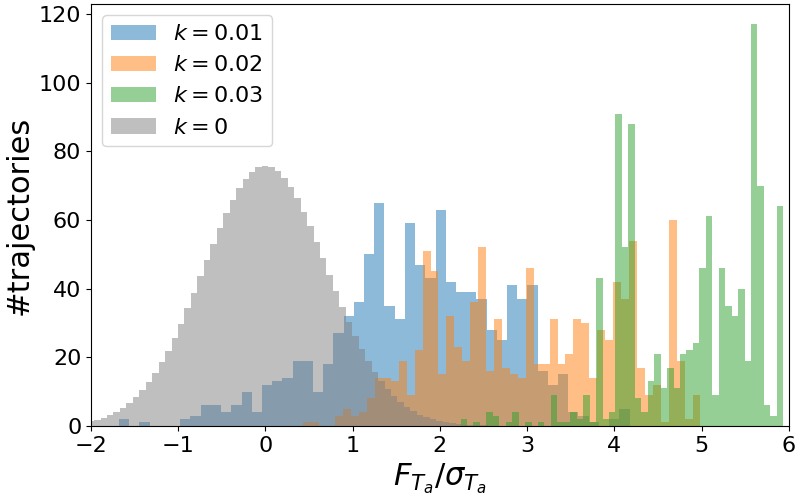
\includegraphics[width=.7\linewidth]{IS_GKTL/IS_GKTL_2}
  \caption{Histogram of the values of the time-averaged drag $F_{T_a}$, with $T_a = 10\tau_c$, in the ensemble sampled by the cloning algorithm, for three values of the cloning strength $k$. In each case, the algorithm was applied with $N=1024$, $\tau = \tau_c / 2$. The grey histogram represents the average histogram obtained through a direct sampling, \textit{i.e.} with $k=0$. It was computed using a Gaussian approximation for the \ac{pdf} of the time-averaged drag.}
  \label{fig:IS_GKTL}
\end{figure}
Figure~\ref{fig:IS_GKTL} shows the histogram of the values of the average drag $F_{T_a} = \frac{1}{T_a}\int_{0}^{T_a}f_d(t)\mathrm{d}t$ for three ensemble of trajectories sampled with three different values of the cloning strength $k$.
It illustrates that the algorithm effectively samples preferentially trajectories with a higher value of the average.
The higher $k$, the stronger the bias.
The grey histogram represents the average histogram that would be obtained using a direct approach -- \textit{i.e.} with $k=0$ -- for the same computational cost.
We computed this histogram by approximating the \ac{pdf} of the drag averaged over $10\tau_c$ as a Gaussian \ac{pdf} (see figure~\ref{fig:PDF_AVG}).
Figure~\ref{fig:IS_GKTL} also illustrates that the sampling by the algorithm is very concentrated on some fluctuations values, and that this effect increases as $k$ increases.
This results from the overlap of trajectories as a consequence of the cloning and pruning.
Indeed, if a trajectory is cloned at step $i$, then the trajectory ${\mathbf{x}(t)}$ over the interval $[0;i\tau]$ will be the same for all the clones.
For a fixed ensemble size $N$, the overlap of trajectories increases as $k$ increases as fewer
trajectories are cloned into a higher number of duplicates.
\textbf{How do we quantify this effect? It is probably application-dependant. What are the strategies to mitigate it?}

Figure~\ref{fig:timeseries_extrms_AVG_GKTL} displays the drag timeseries for several trajectories within the ensemble sampled by the cloning algorithm.
It illustrates that the cloning algorithm samples trajectories that exhibit successive positive fluctuations, resulting in a very large value of the average drag.
Note that during the post-processing of the sampled trajectories, trajectories overlapping over more than half of their duration ($5 \tau_c$) have been considered duplicates, and treated as effectively the same trajectory.
This procedure resulted in an ensemble of ?? "distinct" trajectories (out of the original $N = 1024$).

\begin{figure}
  \centering
  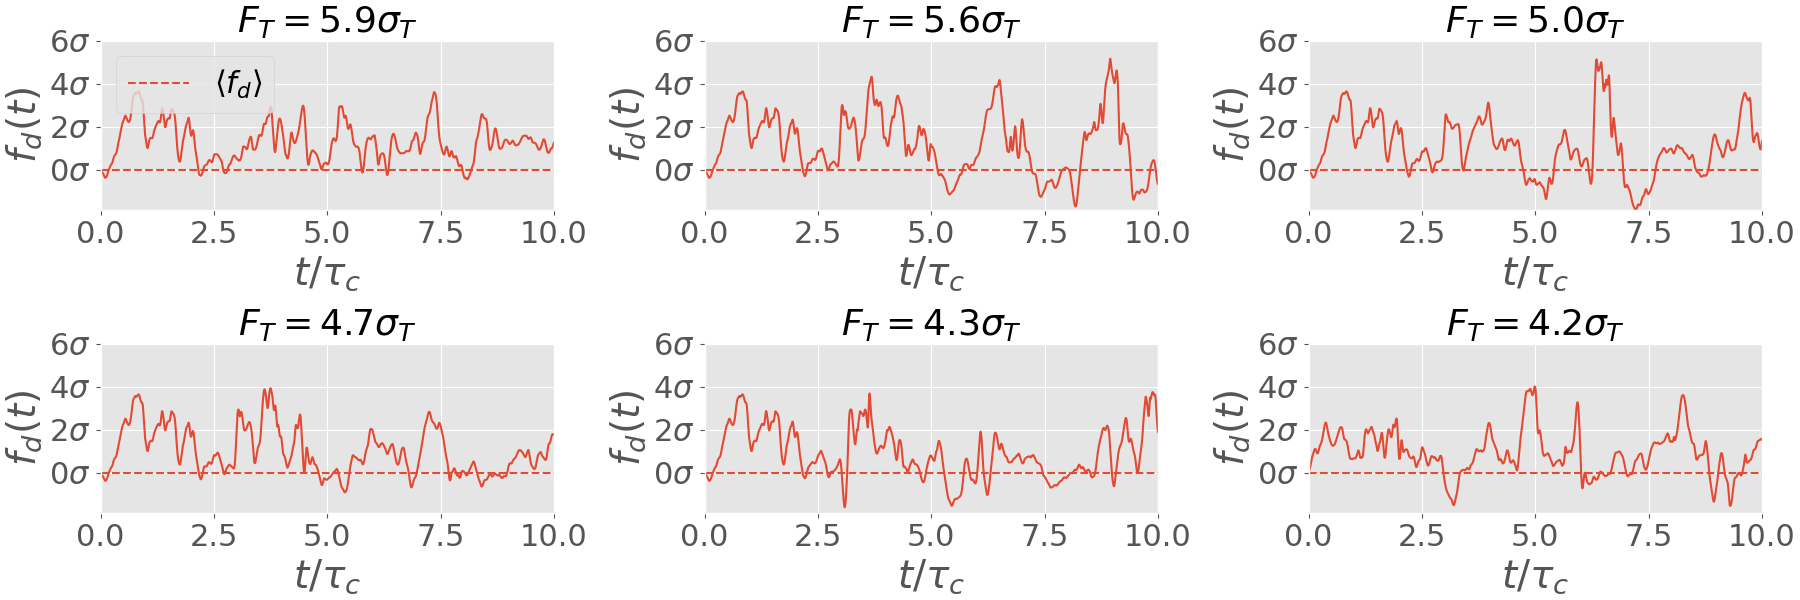
\includegraphics[width=\linewidth]{timeseries_extrms_AVG_GKTL/timeseries_extrms_AVG_GKTL}
  \caption{Drag timeseries corresponding to the 6 highest fluctuations of the average drag in the ensemble sampled by the cloning algorithm. The cloning algorithm was applied with $N = 1024$, $\tau = \tau_c / 2$ and $k = 0.03$. }
  \label{fig:timeseries_extrms_AVG_GKTL}
\end{figure}

In addition, figure~\ref{fig:illustr_extrms_vorticity_GKTL} displays the vorticity field at the time of maximum drag over a subset of trajectories
sampled by the cloning algorithm.
It shows that the sampled events are consistent with the picture of strong vorticity levels being concentrated in the vicinity of the base of the obstacle, as pointed out in section~\ref{sec:instantaneous_drag}.
Moreover, we stress that the computational cost for the sampling of the events shown in figures~\ref{fig:timeseries_extrms_AVG_GKTL} and~\ref{fig:illustr_extrms_vorticity_GKTL} is roughly a hundredth of computational cost of the direct sampling required to sample events shown in figures~\ref{fig:extreme_avg} and~\ref{fig:top_4_events_vorticity}.

\begin{figure}
  \centering
  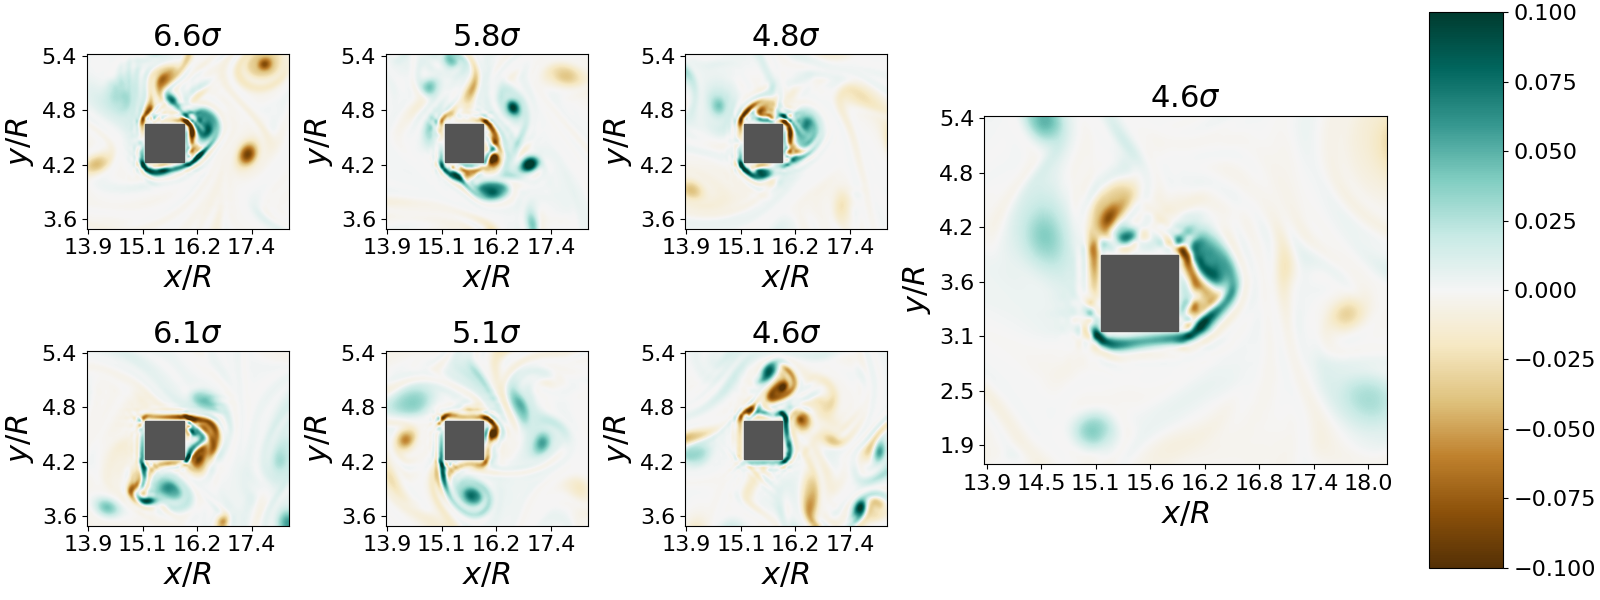
\includegraphics[width=\linewidth]{illustr_extrms_vorticity_GKTL/illustr_extrms_vorticity_GKTL}
  \caption{Vorticity field corresponding the maximum of the drag $f_d$ over trajectories sampled by the cloning algorithm.}
  \label{fig:illustr_extrms_vorticity_GKTL}
\end{figure}

An important remaining question is whether or not the sampled ensemble of trajectories are representative of the full range of dynamics that can lead to extreme values of the average drag.
Indeed, it was observed in section~\ref{sec:time_avg} that large values of the average drag over $10\tau_c$ can result from a variety of different
dynamics, including the succession of independent positive fluctuations, but also the occurrence of fewer and larger fluctuations separated by periods of typical drag.
In particular, it is not clear from the results of the present work whether or not the cloning algorithm is suited to sample trajectories of the latter form.
A possible continuation of this study is to go beyond the qualitative description of the events sampled by the cloning algorithm, a task that is left to future work.

\subsubsection{Computation of return times}
\label{sec:return_times}

Beyond dynamical aspects, the cloning algorithm provides ensemble of trajectories over which statistics of rare events can be computed by inverting Eq.~\eqref{eq:Biased_Path_Approximation_main}.
In this section, we show that the biased sampling performed by the cloning algorithm allows for the computation of return times for events otherwise out-of-reach from a direct sampling approach.

Each trajectory $j$ in the biased ensemble results in a timeseries of the time-averaged drag:
\begin{equation}
\label{eq:time_averaged}
F_T^{(j)}(t) = \int_{t-T}^{t}f_d^{(j)}(\tau)d\tau, \quad t\in [T,T_a]  ,
\end{equation}
and the return time of a fluctuation $F_T \geq a$ is given by~\citep{lestang_computing_2018}
\begin{equation}
r(a) = - \frac{T_a - T}{\ln (1-\mathbb{P}(F_T \geq a))}.
\end{equation}


The probability $\mathbb{P}(F_T \geq a)$ can be estimated from the biased ensemble by inverting Eq.~\eqref{eq:Biased_Path_Approximation_main}
\begin{equation}
  \mathbb{P}(f_d \geq a) \approx \frac{1}{N}\sum_{j=1}^{N}e^{T_a \lambda(k)}e^{kT_aF_T^{(j)}}s_j(a),
\end{equation}
with $s_j(a) = 1$ if $\max_{T\leq t \leq T_a}[F_T^{(j)}] \geq a$ and $s_j(a) = 0$ otherwise. This amounts to taking the sum of the weights of the timeseries which maximum is larger than $a$.

Fig.~\ref{fig:return_times_gktl} displays the return times for extreme fluctuations of the time-averaged drag acting on the square obstacle.
Two independent estimates are shown, obtained using different values of the cloning strength $k$.
Note that both estimates have been computed with the same computational cost $T_{tot}=N\times T_a$.
In addition, figure~\ref{fig:return_times_gktl} shows an estimate computed through direct sampling with the same computational cost, \textit{i.e.} using a timeseries of duration $T_{tot}$.
Whilst a direct approach cannot access events with a return time greater than $T_{tot}$, the cloning algorithm allows for the computation of statistics of drag fluctuations having a return time several orders of magnitude above $T_{tot}$.
This result shows that the biased ensemble sampled by cloning algorithm enables the estimation of return times for average drag fluctuations that would be out-of-reach from a direct sampling.
Alternatively, for a fixed target return time, the use of the cloning algorithm can reduce the computational cost of the estimation by several orders of magnitude.
This is obviously a major advantage of this rare-event sampling algorithm.

More generally, the successful computation of return times indicates that, despite the complex dynamics and the overlapping trajectories, the biased ensemble generated by the cloning algorithm may be used to compute statistical estimators in a very efficient manner.
We note, however, that some estimators may be more affected by the quality of the sampling than others.

\begin{figure}
  \centering
  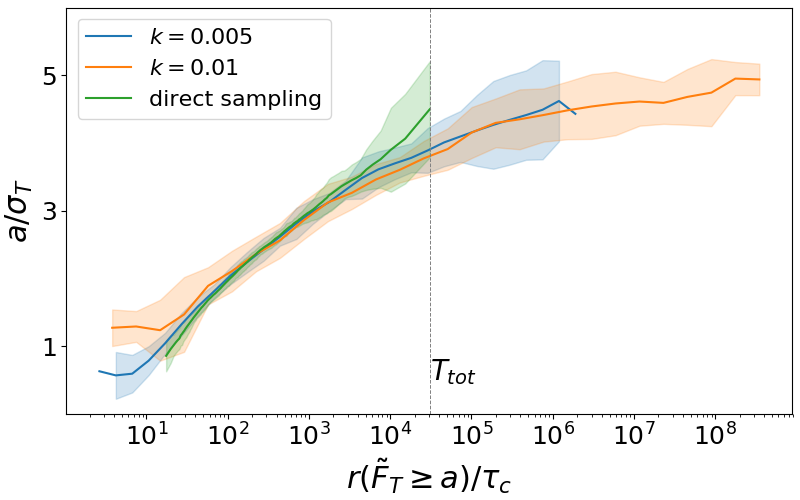
\includegraphics[width=.7\linewidth]{return_times_GKTL/return_times_GKTL}
  \caption{\label{fig:return_times_gktl} Return times for the time-averaged drag acting on the square obstacle. $\tilde{F}_T$ denotes the time-averaged drag with zero mean. The blue and red lines are obtained from the biased ensemble of trajectories generated by the \ac{gktl} algorithm with $N=1024$ and $T_a=30\tau_c$. The green line is the return times obtained from a single timeseries of duration equal to the computational cost of both \ac{gktl} experiments. Uncertainty ranges for the \ac{gktl} estimates are computed as the standard deviation over a set of 10 independent experiments. Uncertainty ranges for the direct estimation are computed as the standard deviation over a ensemble of direct estimates resulting from 60 independent timeseries.}
\end{figure}


%%% Local Variables:
%%% mode: latex
%%% TeX-master: "draft_p2_jfm"
%%% End:


\section{Conclusion}
\label{conlusion}

In a first part, we showed that the phenomenology describing extreme drag fluctuations is very different from typical events.
By means of a long simulation of reference, we observed that such extreme events are caused by the (temporary) trapping of vorticity very close to the base of the square.
The lifetime of extreme drag fluctuations of the order of the turnover time, and the corresponding drag signal is very peaked around these extreme values.
Furthermore, this lifetime is of the order of the correlation timescale of the drag and therefore each successive extreme drag events are decorrelated for one another.
From a timeseries spanning four million turn-over times we also illustrated that the phenomenology of extremes of the time-averaged drag cannot be reduced to a well defined scenario.
Indeed, extreme average values result both from rare successions of typical fluctuations, of the occurrence a fewer number of rare extreme fluctuations of the instantaneous drag.

In order to extend our study, and consider its replication on more complex flows, we considered the application of two popular rare-event sampling algorithms.
Because of the short lifetime of extreme drag fluctuations, the \ac{ams} does not lead to a better sampling
when using the drag itself as a score function.
The choice of the score function is difficult for complex dynamics, and optimal score function is problem-dependant.
To enable the application of the \ac{ams} to a wide range of complex dynamical systems, an important question is the systematic estimation of the optimal score function, for instance using machine learning approaches.

We obtained more satisfactory results for the averaged drag using the \ac{gktl} algorithm.
Indeed, using the algorithm we could sample trajectories corresponding to values of the time-averaged drag unreachable from a direct sampling of similar computational cost.
Qualitatively, we found the phenomenology of the sampled extreme events to be consistent with the findings of the part of the study.
However, a more quantitative analysis is required to assess the ability of the \ac{gktl} algorithm to equally sample the different dynamics leading to a given extreme value of the average drag.
Nonetheless, our study shows that the sampled ensemble is useful to compute estimators over extreme events, such as return times of extreme fluctuations of the average drag.

\section{Acknowledgements}
The authors thank Francesco Ragone, Corentin Herbert, Charles-Edouard Bréhier and Eric Simonnet for useful discussions and suggestions on various aspects of this work.
T.L and F.B acknowledge support from the European Research Council under the European Union's seventh Framework Program (FP7/2007-2013 Grant Agreement No. 616811).
Simulations have been performed on the local HPC facilities at École Normale Supérieure de Lyon (PSMN) and École Centrale de Lyon (PMCS2I).
The facilities at PSMN are supported by the Auvergne-Rhône-Alpes region (GRANT CPRT07-13 CIRA) and the national Equip@Meso grant (ANR-10-EQPX-29-01).
Finally, the authors would like to thank the three anonymous referees for their detailed review and insightfull comments and suggestions.

\appendix

\section{The \acl{lbm}}
\label{app:lbm}

% details about LBM
In the LB method, the fluid is viewed as a population of particles that collide, redistribute and propagate along the different links of a discrete lattice (see \cite{kruger_lattice_2017} for a comprehensive introduction).
In our two-dimensional situation, the so-called D2Q9 lattice with only nine possible velocities $\{\mathbf{c_i}\}_{i=0...8}$ at each node has been adopted (see  Fig.~\ref{fig:D2Q9}).
Locally, the macroscopic flow variables (per unit volume) are recovered by summing over the densities of particles $\{f_i\}_{i=0...8}$ moving with the different velocities, i.e.
\[
\rho(\mathbf{x},t) = \sum_i f_i(\mathbf{x},t) \quad \mathrm{and}\quad \rho(\mathbf{x},t) \mathbf u(\mathbf{x},t) = \sum_i f_i(\mathbf{x},t) \mathbf{c_i}
\]
for the mass density and the fluid momentum respectively. The assumption of weak compressibility (for an ideal gas) is made so that the pressure is directly proportional to the mass density: $p = c_s^2 \rho$ where $c_s$ is interpreted as a speed of sound.

\begin{figure}
	\centering
	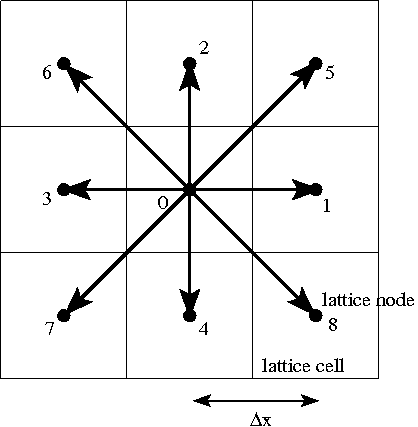
\includegraphics[width=0.3\linewidth]{D2Q9/D2Q9}
	\caption{Sketch of the D2Q9 lattice. Particles move exactly from a lattice node towards one of its nine neighbours (including the node itself) during one time step. By definition, the lattice spacing is related to the time step by $\Delta x/ \Delta t = \sqrt{3} c_s$ where $c_s$ is interpreted as a speed of sound.}
	\label{fig:D2Q9}
\end{figure}


% algo
%
The complexity of the flow emerges from the repeated application of simple rules of streaming and collision. The \ac{lbm} advances the local densities of particles $f_i(\mathbf{x},t)$ moving with velocities $\mathbf{c}_i$  in a two-step procedure. Namely, an \emph{exact} streaming step
\begin{equation}
  \label{eq:lbe}
  f_i(\mathbf{x}+\mathbf{c}_i \Delta t, t + \Delta t) = f_i^{\mathrm{out}}(\mathbf{x},t)
\end{equation}
during which particles move with their own velocity to a neighbouring node, and an instantaneous collision step
\[
f_i^{\mathrm{out}}(\mathbf{x},t) = -\frac 1 {\tau_\nu} \left(f_i(\mathbf{x},t) - f_i^\mathrm{eq}(\mathbf{x},t) \right)
\]
which achieves a relaxation of local densities towards an absolute equilibrium (at the macroscopic level). The time-scale $\tau_\nu$ (in lattice unit) is related to the kinematic viscosity of the fluid by
\[
\nu = \left( {\tau_\nu} - \frac 1 2 \right) c_s^2 ~\Delta t
\]
This simplification of the collision kernel is known as the BGK approximation in the kinetic theory of gas \citep{BGK}.
%
The equilibrium function is given by
\begin{equation}
  \label{eq:lbe_eq}
  f_i^\mathrm{eq}(\mathbf{x},t) = w_i  \rho(\mathbf{x},t) \left( 1 + \frac{\mathrm u(\mathbf{x},t) \cdot \mathbf{c_i}}{c_s^2} +
    \frac{u_\alpha(\mathbf{x},t) u_\beta(\mathbf{x},t)({c_i}_\alpha {c_i}_\beta - c_s^2 \delta_{\alpha\beta})}{2 c_s^4} \right),
\end{equation}
with the weight factors $w_0=4/9,~w_{1...4} = 1/9$ and $w_{5...8}=1/36$ for the D2Q9 lattice.
This discrete Lattice Boltzmann scheme is second-order accurate in $\Delta x $ and compliant to the weakly-compressible Navier-Stokes equations with a third-order error in $\mathrm{Ma}=|\mathbf{u}|/c_s$ as the lattice spacing vanishes, i.e. $\Delta x \to 0$ \citep{succi_book}.

As mentioned before, the pressure is directly accessible from the mass density: $p = \rho c_s^2$. The viscous stress is also obtained easily from the densities of particles by
\[
\tau^\mathrm{visc.}_{\alpha \beta} = -\frac{\nu}{\tau_\nu ~ c_s^2 \Delta t} \sum_i  {c_i}_\alpha {c_i}_\beta (f_i - f_i^\mathrm{eq})
\]
so that the total stress expresses as
\begin{equation}\label{eq:def_stress}
\tau_{\alpha \beta} = -  c_s^2 \sum_i f_i ~ \delta_{\alpha\beta}  - \frac{\nu}{\tau_\nu ~ c_s^2 \Delta t} \sum_i  {c_i}_\alpha {c_i}_\beta (f_i - f_i^\mathrm{eq})
\end{equation}
Finally, let us mention that in the present context of turbulent flows, the single-relaxation-time BGK collision has been replaced by a multi-relaxation-time procedure based on central moments with an improved stability \citep{De_Rosis_2016}.

%%% Local Variables:
%%% mode: latex
%%% TeX-master: "draft_p2_jfm"
%%% End:
\newtheorem{theo}{Theorem}

\section{The \ac{ams} algorithm}
\label{app_ams}

This appendix describes the \ac{ams} algorithm, gives a brief summary of the main
mathematical results and discusses its use in practice.
\subsection{Description of the algorithm}
We consider an ensemble of $N$ independent trajectories $\{x_n^{(0)}(t)\}_{1\leq n \leq N}$, for a fixed duration $T_a$.
These trajectories could be generated by any continuous time Markov model: a stochastic process, for instance a diffusion, or a chaotic deterministic dynamical system.

Starting from this initial ensemble, the \ac{ams} consists in a series of iterations in which one or more trajectories are discarded, and re-simulated from a given point in time $t \in [0, T_a]$ to the final time $t = T_a$.

To start off with, each of these trajectories is associated a weight $w_0=1$.
Then, at iteration $j\geq 1$, we evaluate the score of all trajectories $\{x_n^{(j-1)}(t)\}_{1 \leq n \leq N}$ at iteration $j-1$, measured by the maximum of the score function $\xi$ over the whole trajectory:
\begin{equation}
  \mathcal{Q}_n^{(j)} = \sup_{0 \leq t \leq T_a} \xi(t,x_n^{(j-1)}(t)).
\end{equation}
Then, the trajectories corresponding to the lowest $\mathcal{Q}_n^{(j)}$ are selected: we denote $\mathcal{Q}_j^\star= \min_{1\leq n \leq N} \mathcal{Q}_n^{(j)}$ and $n_{j,1}^\star,\ldots,n_{j,\ell_j}^\star$ the indices of trajectories such that:
\begin{equation}
  \label{eq:ams_threshold_def}
  \mathcal{Q}_{n_{j,1}^\star}^{(j)} = \cdots = \mathcal{Q}_{n_{j,\ell_j}^\star}^{(j)} = \mathcal{Q}_j^\star.
\end{equation}
One might expect intuitively that $\ell_j=1$.
However, because of the discretization of the dynamical equations in the numerical model, two or more trajectories may yield the same level $\mathcal{Q}_n^{(j)}$, see~\cite{Brehier2016a}.
The next step is known as the \textit{mutation step}: for each trajectory $x_{n_{j,\ell}^\star}^{(j-1)}$ ($1 \leq \ell \leq \ell_j$), we choose a trajectory $x_{n_\ell}^{(j-1)}$ ($n_{\ell} \neq n_{j,1},\ldots n_{j,\ell_j}$) randomly among the $N-\ell_j$ remaining trajectories, and define the time $t_{j,\ell}$ defined as the smallest time $t$ such that $\xi(t,x_{n_\ell}^{(j-1)}(t))>\mathcal{Q}_j^\star$.
Finally, we define the new replica $x_{n_{j,\ell}^\star}^{(j)}$ by copying the trajectory $x_{n_\ell}^{(j-1)}$ from $t_0$ to $t_{j,\ell}$, and simulating the rest of the trajectory, from $t_{j,\ell}$ to $T_a$.
For a Markov process, for instance a diffusion, a new realisation of the noise is used in order to simulate the new trajectory from $t_j$ to $T_a$.
For a chaotic deterministic system, a small amplitude noise is added to the initial condition at time $t_j$.
The other trajectories are not modified: $x_n^{(j)}=x_n^{(j-1)}$ for $n \neq n_{j,1}^\star,\ldots,n_{j,\ell}^\star$.
The selection-mutation process is illustrated on Fig.~\ref{fig:AMS_schema}.

\begin{figure}
  \centering
  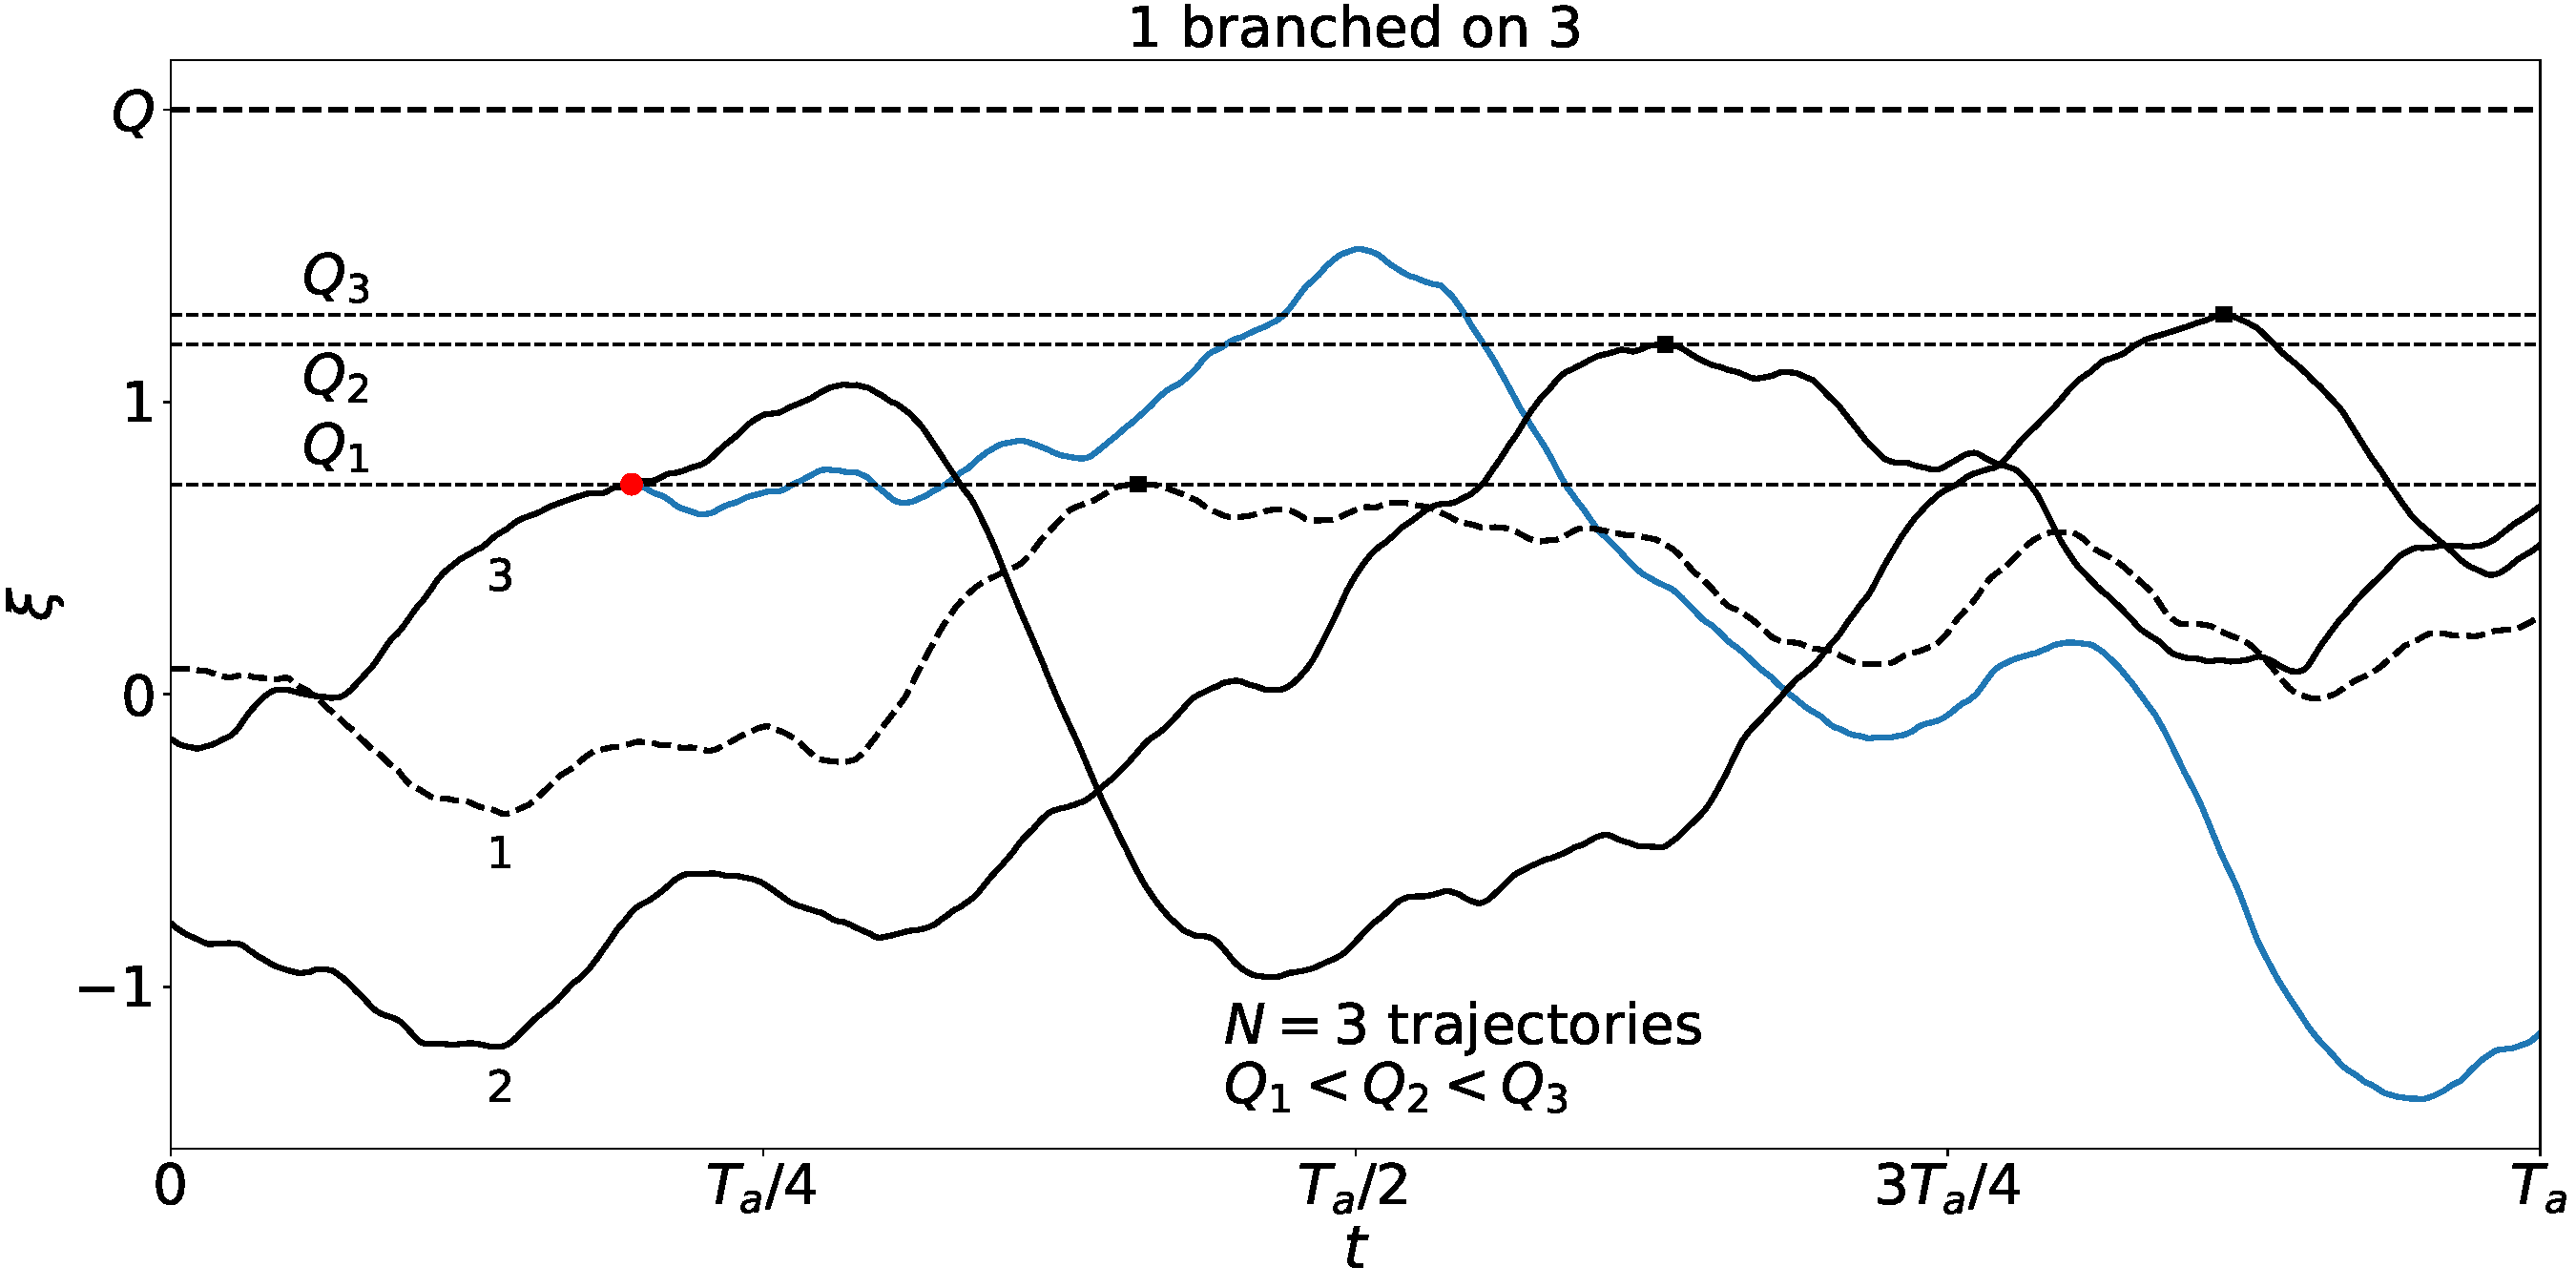
\includegraphics[width=.7\linewidth]{illustr_AMS/illustr_AMS}
  \caption{Illustration of one iteration the \ac{ams} algorithm. Starting from an initial ensemble of 3 trajectories, trajectory 1 is selected as it corresponds to the lowest maximum of the score function $Q_1 = \mathcal{Q}_{j}^\star$. Out of the 2 other trajectories, trajectory 3 is chosen randomly (with probability 1/2) to serve as the base of the resampling of trajectory 1. Trajectory 1 is first made a copy of trajectory 3 from $t=0$ to $t_j$, then simulated from $t_j$ to $T_a$.}
  \label{fig:AMS_schema}
\end{figure}

After $N$ iterations of this selection-mutation procedure, the number of resampled trajectories is
$\tilde{J} = \sum_{j=1}^J \ell_j$.
Ultimately, the algorithm generates $M=N+\tilde{J}$ trajectories, given explicitly by the set $\{x_n^{(0)}\}_{1 \leq n \leq N} \cup \{ x_{n_{j,\ell}^\star}^{(j)}\}_{1 \leq \ell \leq \ell_j, 1 \leq j \leq J}$, or equivalently, the set $\{x_n^{(J)}\}_{1 \leq n \leq N} \cup \{ x_{n_{j,\ell}^\star}^{(j-1)}\}_{1 \leq \ell \leq \ell_j, 1 \leq j \leq J}$.
\subsection{How to compute the probability}
Trajectories $x_n^{(j)}$ forming the ensemble at step $j$ are attributed a weight $w_j$ given by~\cite{Cerou2007,Cerou2011,Brehier2016a}:
\begin{equation}
  w_j = \prod_{i=1}^j \left( 1 - \frac{\ell_i}{N}\right)=\left( 1 - \frac{\ell_j}{N}\right)w_{j-1}.
\end{equation}
This means that each trajectory in the sampled ensemble has an associated weight, given by the iteration until which it was a member of the ensemble: $w_J$ for the final trajectories $\{x_n^{(J)}\}_{1 \leq n \leq N}$, and $w_{j-1}$ for the trajectories $\{ x_{n_{j,\ell}^\star}^{(j-1)}\}_{1 \leq \ell \leq \ell_j, 1 \leq j \leq J}$ resampled at iteration $1 \leq j \leq J$.
Alternatively, $w_0 = 1$ for the initial trajectories, and $w_j$ for the trajectories $\{ x_{n_{j,\ell}^\star}^{(j)}\}_{1 \leq \ell \leq \ell_j, 1 \leq j \leq J}$ resampled at iteration $1 \leq j \leq J$.
Let us relabel these trajectories and their associated weights as $\{(x_m,w_m)\}_{1 \leq m \leq M}$.
Normalising the weights with $W=\sum_{m=1}^M w_m$, we obtain the probabilities $p_m=w_m/W$ associated with the trajectories.
\subsection{Summary of mathematical results}
We now consider the final ensemble of trajectories sampled by the \ac{ams} algorithm, after a given number
of iterations $N$.
We call $a$ the lowest maximum among the trajectories in the ensemble, \textit{i.e.} the final value of the threshold $\mathcal{Q}^{\star}$ defined in Eq.~\eqref{ams_threshold_def}.
The \ac{ams} provides an estimator of the probability that a the maximum of the score function over a trajectory of duration $T_a$ is above $a$, that is:
\begin{equation}
  \label{eq:estimator_ams}
  q(a) = \mathbb{P}\left[ \underset{0\leq t \leq T_a}{\max} \xi(\mathbf{x}, t) > a \right]
\end{equation}
In the following we denote this estimator $\hat{q}_N(a)$.
One of the main properties of the \ac{ams} algorithm is the following unbiasedness result, see~\cite{Brehier2016a} for more general statements, and discussion on the influence of the time discretization of the Markov dynamics.
\begin{theo}
  For every $N$, for every score function $\xi$, $\hat{q}_N$ is an unbiased estimator of $q$:
  \begin{equation}
    \mathbb{E}[\hat{q}_N]=q.
  \end{equation}
\end{theo}
Thus only the statistical error $\text{Var}(\hat{q}_N)$ depends on the choice of $N$, and, more importantly, on the score function $\xi$; see~\cite{Brehier2016a,Rolland2015} for extensive numerical simulations concerning the role of the score function.

More precisely, it is proved in~\cite{Cerou2016}, that the estimator $\hat{q}_N$ satisfies a Central Limit Theorem,
\begin{equation}
  \sqrt{N}\bigl(\hat{q}_N-q\bigr)\underset{N\to \infty}\to\mathcal{N}(0,\sigma^2(\xi,q)),
\end{equation}
with an asymptotic variance $\sigma^2(\xi,q)\in [-q^2\ln q,2q(1-q)]$.
The minimal variance $-q^2\ln q$ is obtained when choosing
\begin{equation}
  \bar{\xi}(t,x;T_a,a)=\mathbb{P}_{x,t}\left\lbrack\underset{t\le s\le T_a}\max O[X,s] > a\right\rbrack,
  \label{eq:time_dependent_committor}
\end{equation}
for all $(t,x)\in[0,T_a]\times \mathbb{R}^d$, where we denote $\mathbb{P}_{x,t}$ the probability over the process initialised at position $x$ at time $t$, and the threshold $a$ and trajectory duration $T_a$ are fixed parameters.


\subsection{How to use it in practice}
In practice, the optimal score function $\overline{\xi}$, also referred to as the \emph{committor}, is of course not known: it is the output of algorithm.
Indeed, $q(a) = \bar{\xi}(0, x_0;T_a,a)$, where $x_0$ denotes an initial condition drawn according to the stationary measure of the dynamics.
Therefore, a crucial point to implement the \ac{ams} is to choose a score function that provides a good approximation of the committor.

Another parameter of the algorithm is the duration $T_a$.
This duration must naturally be chosen larger than the timescale of the rare events of interest, and in this work we use $T_a = 5\tau_c$, where $\tau_c$ is the typical duration of extreme drag fluctuations, see section~\ref{sec:instantaneous_drag}.
Furthermore, we (empirically) observed that the sampling does not benefit form much longer trajectories.
This can be explained as follows.
Considering an arbitrary iteration $j$ and calling $t_j$ is the resampling time (the time at which the parent trajectory reaches $\mathcal{Q}^{\star}$, the resampled trajectory will only be decorrelated from its parent
after a time $\tau_L > \tau_c$ (see section~\ref{sec:ams} and appendix~\ref{app:perturb_branching_time}).
As a result, the probability that it exhibits a fluctuation $\xi > \mathcal{Q}^{\star}$ is $\mathbb{P}_{x_0}[\underset{t_j+\tau_L \le t \le T_a}\max \xi(\mathbf{x},t) > a]$, where $\mathbb{P}_{x_0}$ denotes the probability given a random initial condition drawn according to the stationary measure of the dynamics.
This amounts to direct sampling.

Finally, the \ac{ams} experiments presented in this work do not specify a specific number of iterations $J$, neither a target drag threshold $\mathcal{Q}^{\star}$.
Rather, iterations were carried out until all the trajectories in the ensemble overlap.
Ultimately, because of the discretization induced by the numerical model, all trajectories reach the exact same maximum, \textit{i.e.}
\begin{equation}
  \mathcal{Q}_{n_{j,1}^\star}^{(j)} = \cdots = \mathcal{Q}_{n_{j,\ell_j}^\star}^{(j)} = \mathcal{Q}_j^\star. \quad \text{with} \quad l_j = N
\end{equation}
and the iterations stop.
This phenomenon is sometimes referred as the \textit{extinction} of the algorithm.

\subsection{Illustration of the \ac{ams} on a simple case: the \acl{ou} process}
\label{app:AMS_on_OU}

\begin{figure}
  \centering
  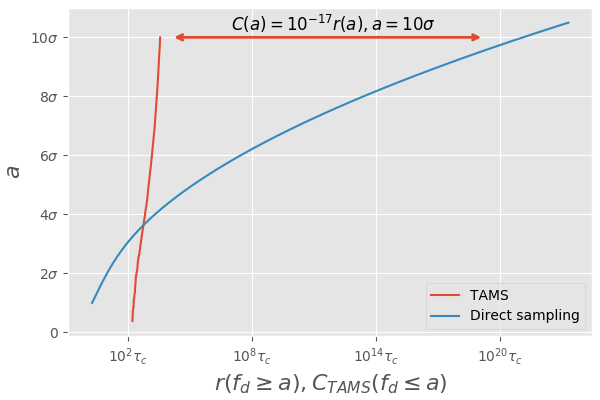
\includegraphics[width=.7\linewidth]{AMS_OU/AMS_OU.png}
  \caption{Efficiency of the \EL{\ac{ams} algorithm} with respect to direct sampling in the case of an Ornstein-Uhlenbeck process \citep{lestang_computing_2018}. The red line represents the evolution of the maximum obtained from re-sampled trajectories as a function of the computational cost $C_{AMS}$. The blue line is the analytical solution for the return time of amplitude $a$.}
  \label{fig:comparaison_temps_de_retour}
\end{figure}
Fluid dynamics is temporarily left aside and a one-dimensional \acl{ou} process is considered:
\begin{equation}
  \label{eq:ou}
  \dot{x} = -x + \eta (t),
\end{equation}
where $\eta$ is a Gaussian noise with $\langle \eta(t)\eta(t-t')\rangle = \delta(t-t')$.
This basic stochastic process will allow us to highlight differences with fluid dynamics.


The \ac{ams} is applied  to a set of $N=32$ trajectories $\{x_n(t)\}_{0\leq t \leq T_a}$ with $T_a=5\tau_c$.
Let us note that the correlation time is $\tau_c = 1$ for the process defined by Eq.~\eqref{eq:ou}.
Our objective is to sample fluctuations $x\geq a$ with $a$ being very large compared to the typical values of $x$.
The score function is simply $x(t)$ and a single trajectory is re-sampled at each iteration.

The computational cost of the algorithm after $J$ iterations is therefore related to the simulation of the $N$ initial trajectories and the re-sampling of $J$ trajectories.
Fig.~\ref{fig:comparaison_temps_de_retour} compares the computational cost of the \ac{ams} algorithm with that of a direct sampling.
In the latter, the typical computational cost is simply the return time $r(a)$.
One can see that the successive re-samplings of the \ac{ams} algorithm lead rapidly to trajectories exhibiting extreme fluctuations.
For large $a$, the computational cost is many orders of magnitude lower than that obtained by direct sampling.

Undoubtedly, the \acl{ou} process has oversimplified dynamics to showcase the efficiency of the \ac{ams} algorithm.
The state space is one-dimensional and the choice of the score function is straightforward: It is $x$ itself.
In addition, the noise term in Eq.~\eqref{eq:ou} has no correlation in time, which implies that newly generated trajectories quickly separate from their parents. Such favorable features \EL{do not} \textit{a priori} persist in the case of fluid dynamics.
  
%%% Local Variables:
%%% mode: latex
%%% TeX-master: "draft_p2_jfm"
%%% End:

\section{The \ac{gktl} algorithm}
\label{app:gktl}
The \ac{gktl} algorithm is based on the simulation of an ensemble of $N$ trajectories $\left\{\mathbf{x}_{n}(t)\right\}_{0\leq t \leq T_a}$ with $ n =1 \cdots N$ starting from independent random initial conditions.
%
Let us consider a real-valued observable of interest $A(\mathbf{x}(t))$, {\emph{e.g.} the drag $f_d(t)$}, and introduce a cloning period $\tau$.
%
At time instants $t_{i}=i\tau$ with $i=1,~2,~...,~T_{a}/\tau$ ($T_{a}$ is a multiple of $\tau$) a weight $W_{n}^{i}$ is assigned to each trajectory. This weight is defined ($t_0=0$) by
%
\begin{equation}
W_{n}^{i}=\frac{e^{k\intop_{t_{i-1}}^{t_{i}}A(\mathbf{x}_{n}(t))dt}}{R_{i}}\quad \mbox{with the normalisation factor} \quad R_{i}=\frac{1}{N}\sum_{n=1}^{N}e^{k\int_{t_{i-1}}^{t_{i}}A(\mathbf{x}_{n}(t))dt}
\label{eq:Weight}
\end{equation}
so that $\sum_{n=1}^N W_n^i = N$.
%
%
{The weights $\{W_{n}^{i}\}_{n=1\cdots N}$ determine how many copies of each trajectory are made at time $t=t_i$. The parameter $k$ characterizes the amplitude of the statistical bias involved in the algorithm (see Fig.~\ref{fig:IS_GKTL}). For more information about the practical implementation of the algorithm, the interested reader can refer to~\cite{brewer2018efficient, lestang:tel-01974316}}.
The application of this re-sampling at each step $t_i$ eventually leads to a biased sampling in the trajectory space; the trajectories corresponding to extreme values of $\int_{0}^{T_a}A(\mathbf{x}_{n}(t))dt$ have a higher probability.
%
The sampled biased distribution writes
%
\begin{align}
\mathbb{P}_{k}\left(\left\{ \mathbf{X}(t)\right\} _{0\leq t\leq T_{a}}=\left\{ \mathbf{x}(t)\right\} _{0\leq t\leq T_{a}}\right) &\underset{N\rightarrow\infty}{\sim} \frac{e^{k\int_{0}^{T_{a}}A(\mathbf{x}(t))dt}}{Z(k,T_a)}\mathbb{\mathbb{P}}_{0}\left(\left\{ \mathbf{X}(t)\right\} _{0\leq t\leq T_{a}}=\left\{ \mathbf{x}(t)\right\} _{0\leq t\leq T_{a}}\right),
\label{eq:Biased_Path_Approximation}
\end{align}
where
$\mathbb{P}_{0}\left(\left\{ \mathbf{X}(t)\right\} _{0\leq t\leq T_{a}} = \left\{ \mathbf{x}(t)\right\} _{0\leq t\leq T_{a}}\right)$
refers formally to the probability of observing the trajectory
$\left\{ \mathbf{x}(t)\right\} _{0\leq t\leq T_{a}}$.
The normalisation factor is given by $Z(k,T_a)=\prod_{i=1}^{T_a/\tau}R_i$.
%
One can mention that
\begin{equation}
\label{eq:mean_field}
Z(k,T_a) \underset{N\to \infty}{\sim} \mathbb{E}_0\left[e^{k\int_{0}^{T_{a}}A(\mathbf{X}(t))dt}\right],
\end{equation}
with $\mathbb{E}_{0}$ being the expectation value with respect to the
distribution $\mathbb{P}_{0}$.
This result relies on the \textit{mean-field approximation}
\begin{equation}
R_{i}=\frac{1}{N}\sum_{n=1}^{N}e^{k\int_{t_{i-1}}^{t_{i}}A(\mathbf{X}_{n}(t))dt}\underset{N\rightarrow\infty}{\sim} Z(k,t_i)= \mathbb{E}_{i}\left[e^{k\int_{t_{i-1}}^{t_{i}}A(\mathbf{X}(t))dt}\right],
\label{eq:Mean_Field_Approximation}
\end{equation}
where $\mathbb{E}_{i}[.]$ denotes the expectation value with respect to the biased distribution $\mathbb{P}_k^{(i)}$ obtained after $i$ cloning steps.
The typical relative error related to this approximation can be shown to be of order $1/\sqrt{N}$ for a family of rare-event algorithms including the \ac{gktl} algorithm~\citep{DelMoralBook,DelMoral2013}.
%
Rejected trajectories are discarded from the statistics.
Eventually, an effective ensemble of $N$ trajectories of duration $T_{a}$ is obtained, distributed according to $\mathbb{P}_{k}$.

A key feature of the \ac{gktl} algorithm is that the sampling procedure does not involve any alteration of the dynamics.
All resampled trajectories are solutions of the original dynamical system.
Nevertheless, it should be noted that a small random perturbation is introduced in the cloning procedure to force clones from the same trajectory to separate, \emph{i.e.} artificial randomness is introduced so that the cloning procedure is effective for deterministic dynamics.
It was checked that this perturbation does not affect the statistics of the sampled trajectories, see appendix~\ref{app:perturb_branching_time}.

Eventually, the sampled trajectories obtained with the \ac{gktl} algorithm can be used to compute the statistical properties of any observable with respect to the distribution $\mathbb{P}_{0}$ from the distribution $\mathbb{P}_{k}$ by using Eq.~\eqref{eq:Biased_Path_Approximation}.

%%% Local Variables:
%%% mode: latex
%%% TeX-master: "draft_p2_jfm"
%%% End:
\section{Perturbation at branching time}
\label{app:perturb_branching_time}
As mentioned in sections~\ref{sec:ams} and~\ref{sec:cloning}, the application of the \ac{ams} and the cloning algorithm to deterministic systems require the the addition of a perturbation to the initial condition of
resampled trajectories.
In the absence of any perturbation, the resampling would not yield new trajectories, but instead exact copies of the trajectories the resampling is based on.

The state of the flow at any point in time is given by the velocity field and the pressure $(\mathbf{u}, p)$, where the dependence on time of both variables is implicit.
A general strategy for perturbing the state of the flow is to construct a perturbative divergence free field $\delta \mathbf{u}$ and corresponding $\delta p$ solution of the
Poisson equation.
In the context of the \ac{lbm} however, the state of the system is described at a mesoscopic level by the ensemble the populations $\{f_k(x_j, y_j)\}_{0\le k \le 8, 0 \le i <N_x, 0 \le j < N_y}$.
A consequence is that, from the knowledge of a macroscopic state ($(\mathbf{u}+\delta \mathbf{u}, p + \delta p)$, it is difficult to obtain the mesoscopic state from with the \ac{lbm} model can be initialised.

In this work we work around this issue by designing the perturbative directly at the level of the mesoscopic populations.
At each lattice site $\mathbf{x}$, the populations ${f_i}_{0\le i \le 8}$ are replaced by
\begin{equation}
  f_{i}(\mathbf{x}) \longrightarrow f_i(\mathbf{x}) + \epsilon \sum_{n=1}^{N} \alpha_{n}f_{i}^{n}(\mathbf{x}), \,\,\, 1\leq i \leq 9,
  \label{eq:perturb_pop}
\end{equation}
with the set $\{\alpha_n\}_{1\leq m \leq N}$ drawn uniformly from $[0,1]$ and $\epsilon$ the amplitude of the perturbation. The perturbed populations are then rescaled so that no mass is added in the system.
For more details concerning this procedure, see appendix C of~\cite{lestang:tel-01974316}
In other words obtained as a linear combination of $N$ solutions $\{f_i^{(n)}\}_{1\le n \le N}(\mathbf{x})$ of the numerical model~\eqref{eq:lbe}.
Note that, the Lattice Boltzmann Equation~\eqref{eq:lbe} is not linear, and therefore a linear combination of solutions can be assimilated as a solution of the numerical model.
However, nonlinearities in~\eqref{eq:lbe} are located in the equilibrium distributions~\eqref{eq:lbe_eq}, and are of order of the Mach number $\mathbf{u}/c_s$ that is kept small compared to $1$, see section~\ref{sec:test_flow}.

\begin{figure}
  \centering
  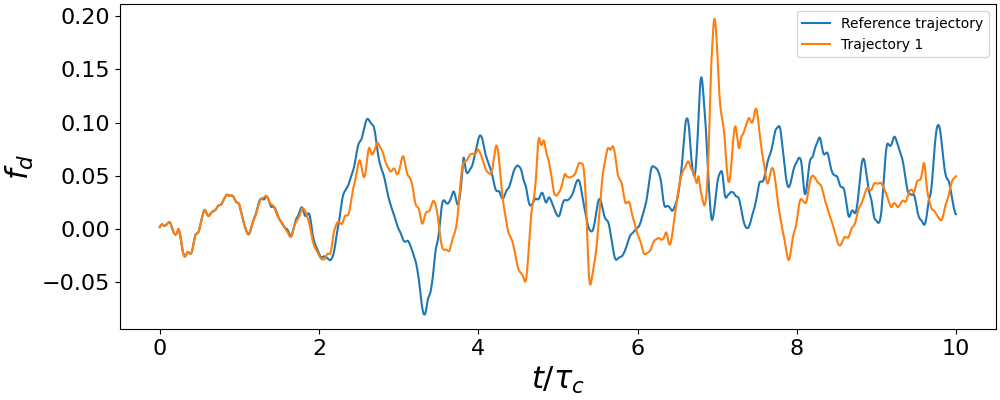
\includegraphics[width=.7\linewidth]{effect_of_perturbation/effect_of_perturbation}
  \caption[Illustration of the perturbation of the initial condition]{The blue line shows the evolution of the drag acting on the obstacle over time for a simulation initialised on a given initial condition. The second line represents the evolution of the drag for a simulation initialised on the same initial condition, however slightly perturbed as described in this appendix. $N=10$, $\epsilon=0.002$}
  \label{fig:effect_of_perturbation}
\end{figure}

In this work, we chose $N = 10$ and $\epsilon = 0.002$.
Figure~\ref{fig:effect_of_perturbation} illustrate the effect of applying a small perturbation on the evolution of the drag acting on the square obstacle.
The value of $\epsilon$ was chosen so that the perturbation does not impact the statistics of the drag.
In order to check this assumption, we generated a timeseries of duration $T_{tot} = 10^5 \tau_c$, and introduced a perturbation with $\epsilon = 0.002$ with a period $\tau = \tau_c / 2$, mimicking the perturbation of clones in the cloning algorithm.
Figure~\ref{fig:pdf_drag_with_perturbation} shows that the correct statistics are obtained even in presence of this slight perturbation.

\begin{figure}
  \centering
  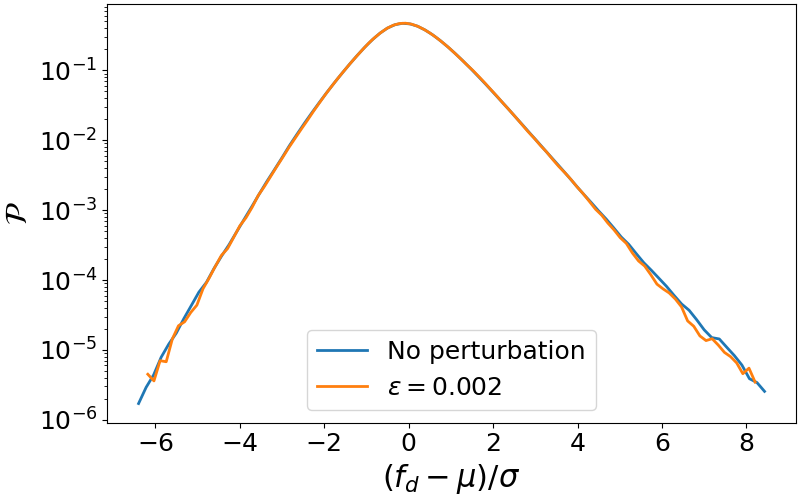
\includegraphics[width=.7\linewidth]{pdf_drag_with_perturbation/pdf_drag_with_perturbation}
  \caption{Estimation of the \ac{pdf} with and without periodic perturbations}
  \label{fig:pdf_drag_with_perturbation}
\end{figure}

%%% Local Variables:
%%% mode: latex
%%% TeX-master: "draft_p2_jfm"
%%% End:


\bibliographystyle{jfm}
\bibliography{../biblio}

\end{document}


%%% Local Variables:
%%% mode: latex
%%% TeX-master: t
%%% End:
